\documentclass{article}
\usepackage{graphicx} % Required for inserting images
\usepackage{titlesec} % Required for customizing section titles
\usepackage{hyperref}
\usepackage{listings}
\usepackage{url}
\usepackage[T1]{fontenc}



% Configure hyperref to make URLs clickable without border or color
\hypersetup{
    colorlinks=true,
    urlcolor=blue,
    linkcolor=blue,
    citecolor=blue,
    filecolor=blue,
    breaklinks=true,
}

% Redefine \section command to include a period after the section number
\titleformat{\section}{\normalfont\Large\bfseries}{Exercise \thesection.}{1em}{}

\title{Security Insider Lab II- SS 2024 \\ First Task}

\author{Sayed Alisina Qaderi (112092) \\ Dusan Dordevic (115556) \\ Atiqullah Ahmadzai (112518)}
\date{April 2024}
\vskip 2\baselineskip
% Add university name, professor's name, and assistant's name
\newcommand{\university}{\textbf{University of Passau}}
\newcommand{\professor}{Prof. Dr. Joachim Posegga}
\newcommand{\assistant}{Talaya Farasat \& Aleena Elsa George}

\begin{document}

\maketitle
\thispagestyle{empty} % Remove the page number from the first page

% University, Professor, and Assistant
\begin{center}
    \university \\
    Professor: \professor \\
    Assistants: \assistant
\end{center}

% Table of Contents
\clearpage
\tableofcontents
\thispagestyle{empty} % Remove the page number from the table of contents page

% Exercise 1
\clearpage

\section{Definitions}\label{owasp}\cite{owasp}


\subsection{SQL injection}
     The SQL injection attack consists of the insertion or “injection” of an SQL query via the input data from the client into the application. A successful SQL injection exploit can read sensitive data from the database, modify database data (Insert/Update/Delete), execute administration operations on the database (such as shutdown the DBMS), recover the content of a given file present on the DBMS file system and in some cases issue commands to the operating system.
     
    SQL injection attacks are injection attacks in which SQL commands are injected into data-plane input to affect the execution of predefined SQL commands. 
    SQL injection attacks typically occur when the user inputs of a web application are not sanitized or validated properly. For instance, the most used generic payloads are the following ASCII characters :
    \begin{itemize}
        \item ''
        \item `
        \item ``
        \item ,
        \item "
        \item ""
        \item /
        \item //
    \end{itemize}
    
\subsection{Cross-site scripting (XSS)}
    Cross-site scripting (XSS) attacks are a type of injection in which malicious scripts are injected into otherwise benign and trusted websites. XSS attacks occur when an attacker uses a web application to send malicious code, generally in the form of a browser-side script, to a different end user.  
    
    Flaws that allow these attacks to succeed are quite widespread and occur anywhere a web application uses input from a user within the output it generates without validating or encoding it. 
    Currently, a variety of XSS attacks can be categorized as follows: 
    \begin{itemize}
        \item Stored XSS attacks 
        \item Reflected XSS attacks.
    \end{itemize}
    The most common payloads are: 
    \begin{itemize}
            \item <script> alert(“Hello XSS”) </script>
            \item <body onload=alert('Hello XSS') />
    \end{itemize}
    If the execution of the arbitrary JavaScript function alert() is successful, the web page is vulnerable to XSS.
    
\subsection{Command injection}
    
        Command injection vulnerability refers to the ability to inject arbitrary code into the target machine. Command injection has various use cases, and it is used to compromise vulnerable software that is running on a targeted host. The probability of occurrence regarding this vulnerability is low. 
        However, it can lead to potential system takeover and reverse shell if abused correctly.
    
\subsection{Cross-site request forgery (XSRF)}
    
        CSRF or XSRF stands for Cross-Site Request Forgery. It's a type of security exploit where an attacker tricks a user into unknowingly executing actions on a website they are authenticated with. 
        
        In a CSRF attack, the attacker's goal is to cause an innocent victim to unknowingly submit a maliciously crafted web request to a website that the victim has privileged access to. This web request can be crafted to include URL parameters, cookies and other data that appear normal to the web server processing the request.  
        
        At risk are web applications that perform actions based on input from trusted and authenticated users without requiring the user to authorize (e.g., via a popup confirmation) the specific action. A user who is authenticated by a cookie saved in the user's web browser could unknowingly send an HTTP request to a site that trusts the user and thereby cause an unwanted action. 
        
        Usually, this attack is executed with malicious URL crafting. 
        The exploit URL can be disguised as an ordinary link, encouraging the victim to click it.
    
\subsection{Path disclosure}

    Path disclosure vulnerabilities occur when a web application or system reveals sensitive information about its file structure or internal paths to an attacker. 
    This information disclosure can happen in various ways, such as error messages, debug output, or direct responses from the application.
    
\subsection{Remote code execution}

        Remote code execution allows the attacker to execute malicious arbitrary code on the target machine remotely thus giving him access to the machine and potentially giving him access to the resources of the machine. RCE, or Remote Code Execution, vulnerabilities are among the most severe security issues a system can face. They allow attackers to execute arbitrary code on a target system remotely, which means they can take full control of the system and potentially access, modify, or delete sensitive data, install malware, or use the system for further attacks. The severity of an RCE vulnerability depends on various factors, including the context in which it occurs, the level of access the attacker gains, and the potential impact on the affected system and its users.

\subsection{Open redirect}

        An open redirect vulnerability occurs when a web application takes a parameter from the user and redirects them to the value of that parameter without proper validation. This can be exploited by attackers to redirect users to malicious websites, phishing pages, or other harmful content. 
        \begin{itemize}
            \item  https:://testwebsite.com/redirect?=https://maliciouswebsite.com
        \end{itemize}     


% Exercise 2
\clearpage
\section{word2vec Embedding}\nocite{vulndetection}
\subsection{\textbf{Creating the Corpus}}

The first step is to create the corpus after cloning the repository from GitHub. We must install the required library for this class, which is \href{https://pydriller.readthedocs.io/en/latest/}{PyDriller}. 
\newline
PyDriller is a Python framework that helps developers on mining software repositories. With PyDriller, you can easily extract information from any Git repository, such as commits, developers, modifications, diffs, and source codes, and quickly export CSV files. \cite{pydriller}
\newline
PyDriller helps this class extract all commits from the GitHub repositories, which is the essential part of this repository. As mentioned in the exercise sheet, we have extracted all commits with the PyDriller from the following repositories.
\begin{itemize}
    \item \href{https://github.com/numpy/numpy}{NumPy}
    \item \href{https://github.com/django/django}{Django}
    \item \href{https://github.com/scikit-learn/scikit-learn}{sci-kit-learn}
    \item \href{https://github.com/tensorflow/tensorflow}{TensorFlow}
    \item \href{https://github.com/scipy/scipy}{scipy}
    \item \href{https://github.com/pallets/flask}{flask}
    \item \href{https://github.com/sqlmapproject/sqlmap}{sqlmap}
    \item \href{https://github.com/docker/compose}{compose}
\end{itemize}
We must remember that there are some changes in the PyDriller library since it was used for this repository. The changes are as follows:
\begin{enumerate}
    \item The \textit{RepositoyrMinning} class changed to \textit{Repository} \newline \textbf{Repository} is the main class of Pydriller, responsible for returning the list of commits you want. One of the main advantages of using PyDriller to mine software repositories is that it is highly configurable. We will now see all the options one can pass to the Repository.

    \item The \textit{modifications} method of RepositoyrMinning changed to 
        \textit{modified\_files} object. \newline We can get a list of modified files as well as their diffs and current source code from each commit. All Modifications can be obtained by iterating over the ModifiedFile object.
\end{enumerate}

After extracting the data from GitHub repositories, it will be saved in a specific file, \textit{pythontraining.txt} in the w2v. The result is shown in Figure \ref{fig: Figure1}.

\begin{figure}[!ht]
    \centering
    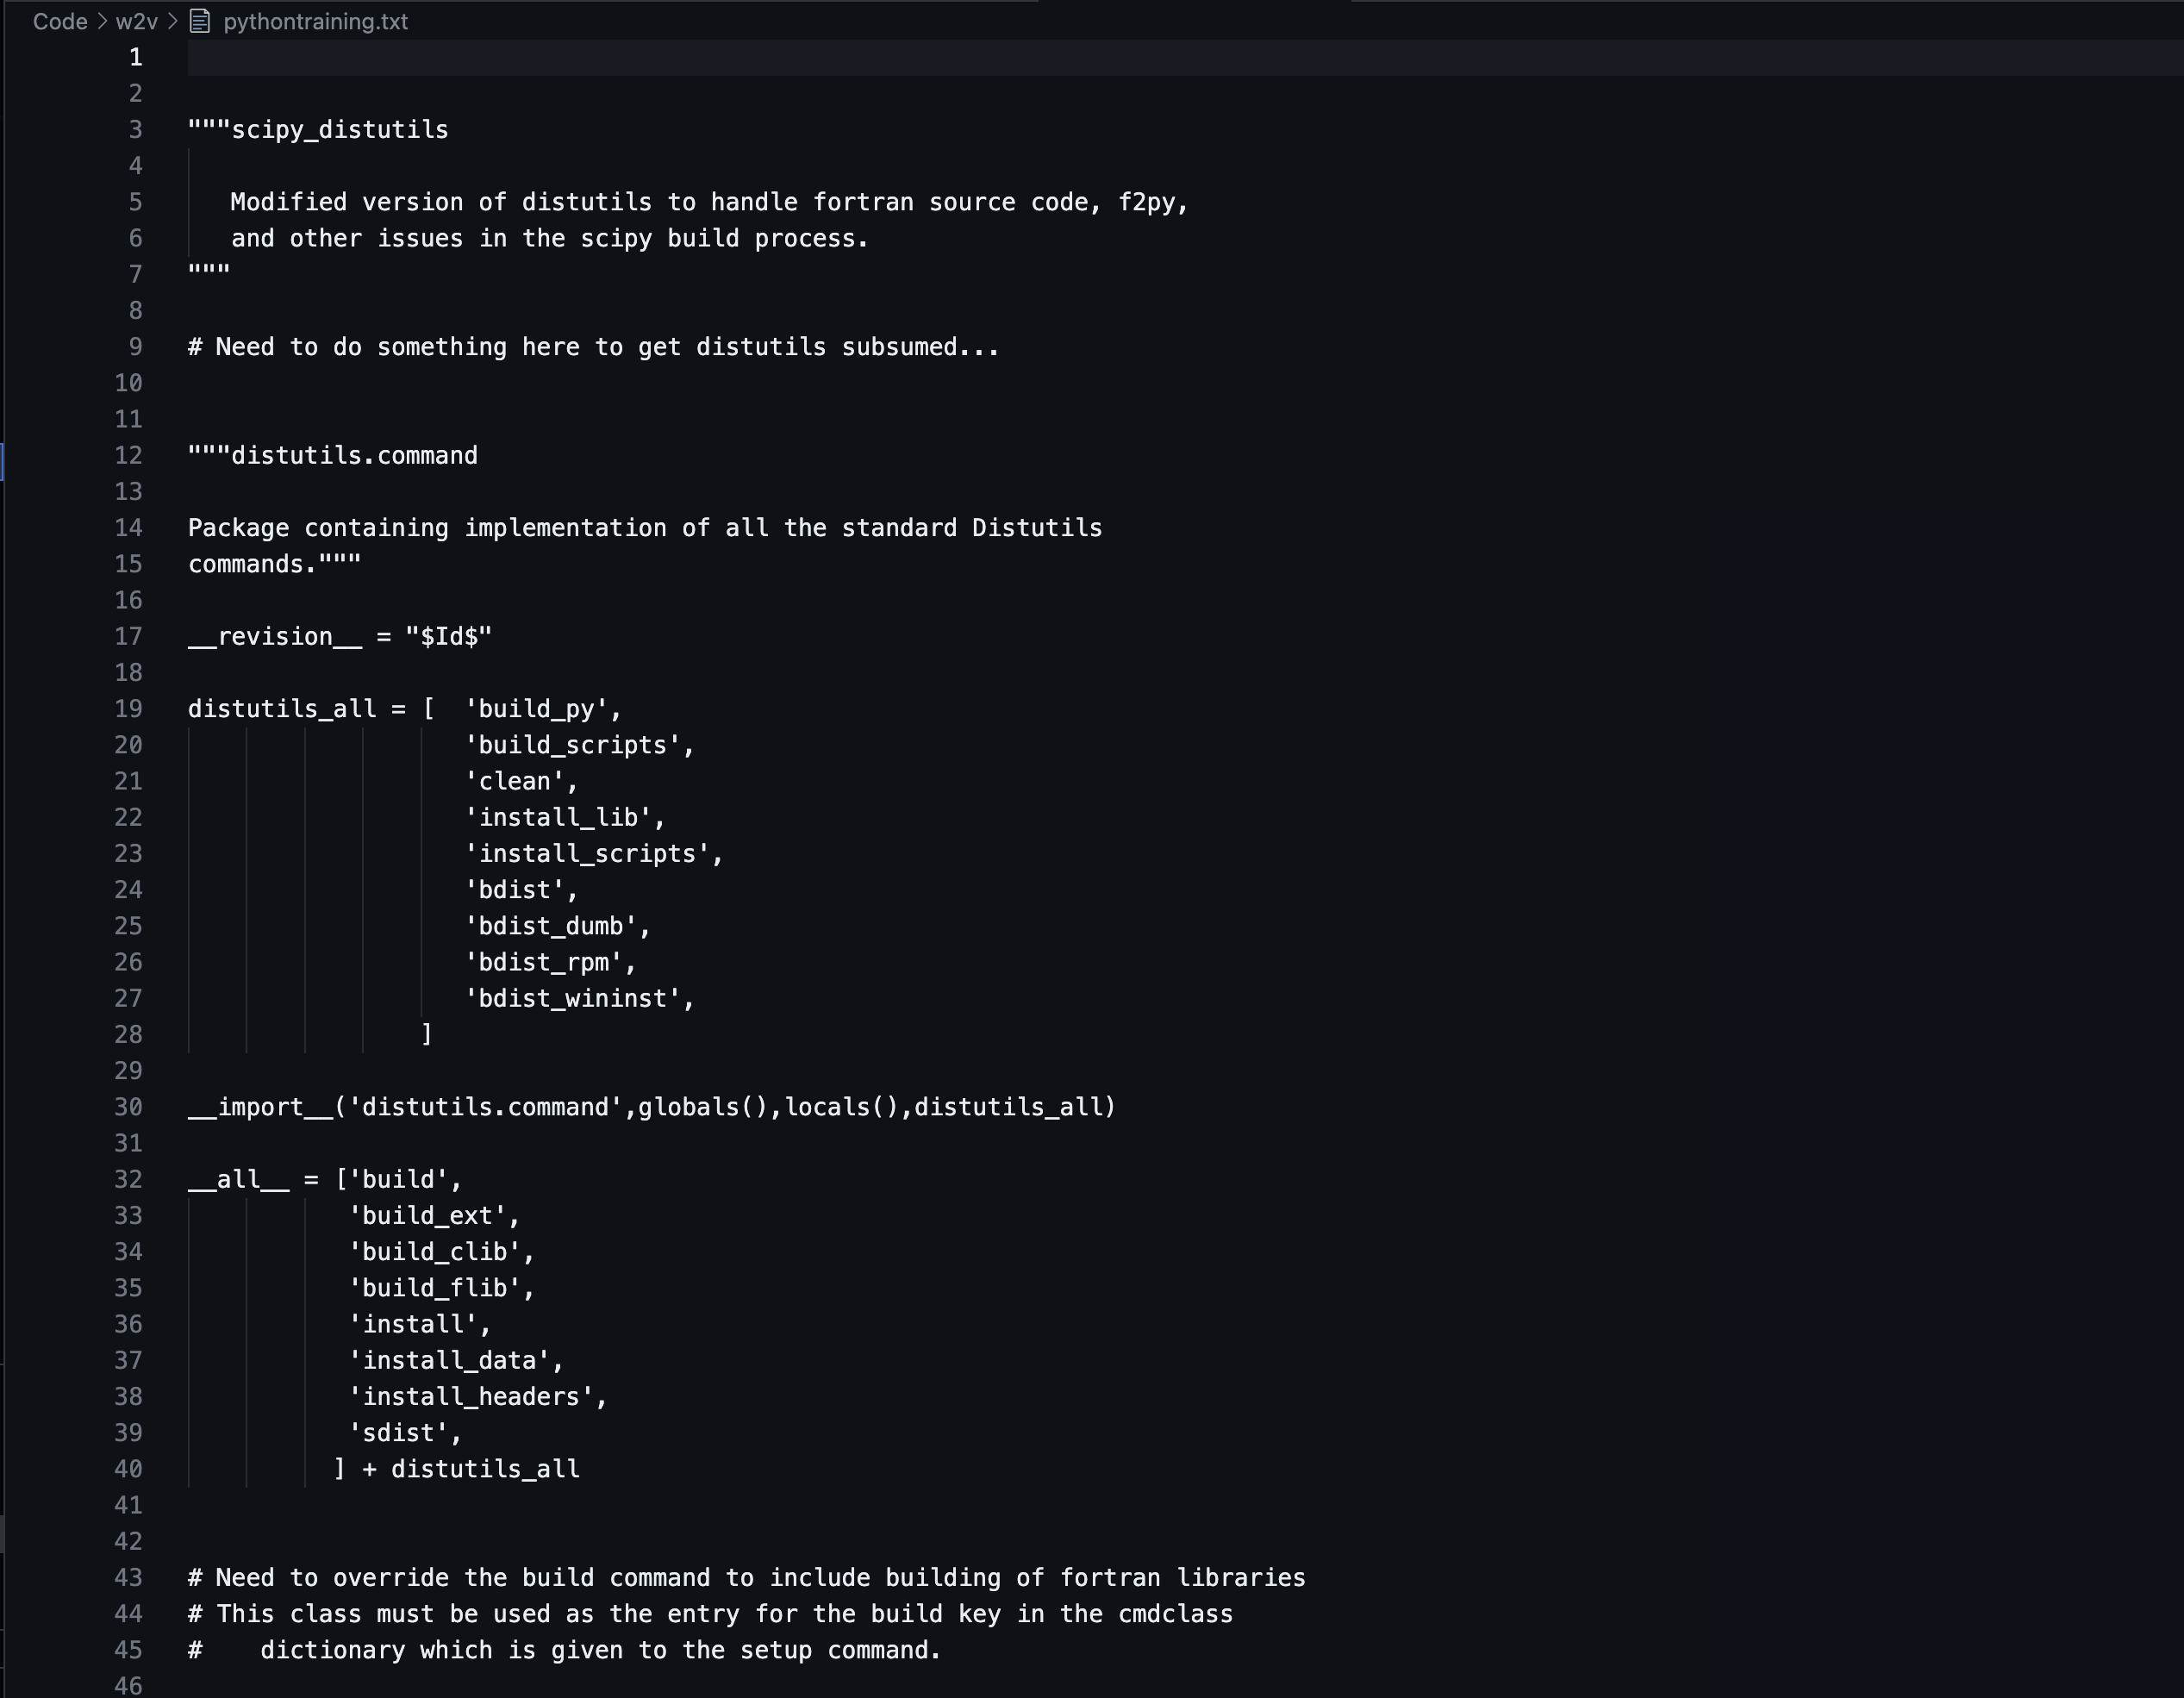
\includegraphics[width=1\linewidth]{pictures/py_training.png}
    \caption{Mined Data From GitHub Repositories}
    \label{fig: Figure1}
\end{figure}

\subsection{\textbf{Fixing Syntax Error}}
We have worked on the "w2v\_cleancorpus.py" file for this part of the task. 
In the mentioned file, we have encountered only one issue: Importing the StringIO library. It is changed from the "StringIO" main library to an "io" library module.\ref{fig: Figure2} 
\begin{figure}[!ht]
    \centering
    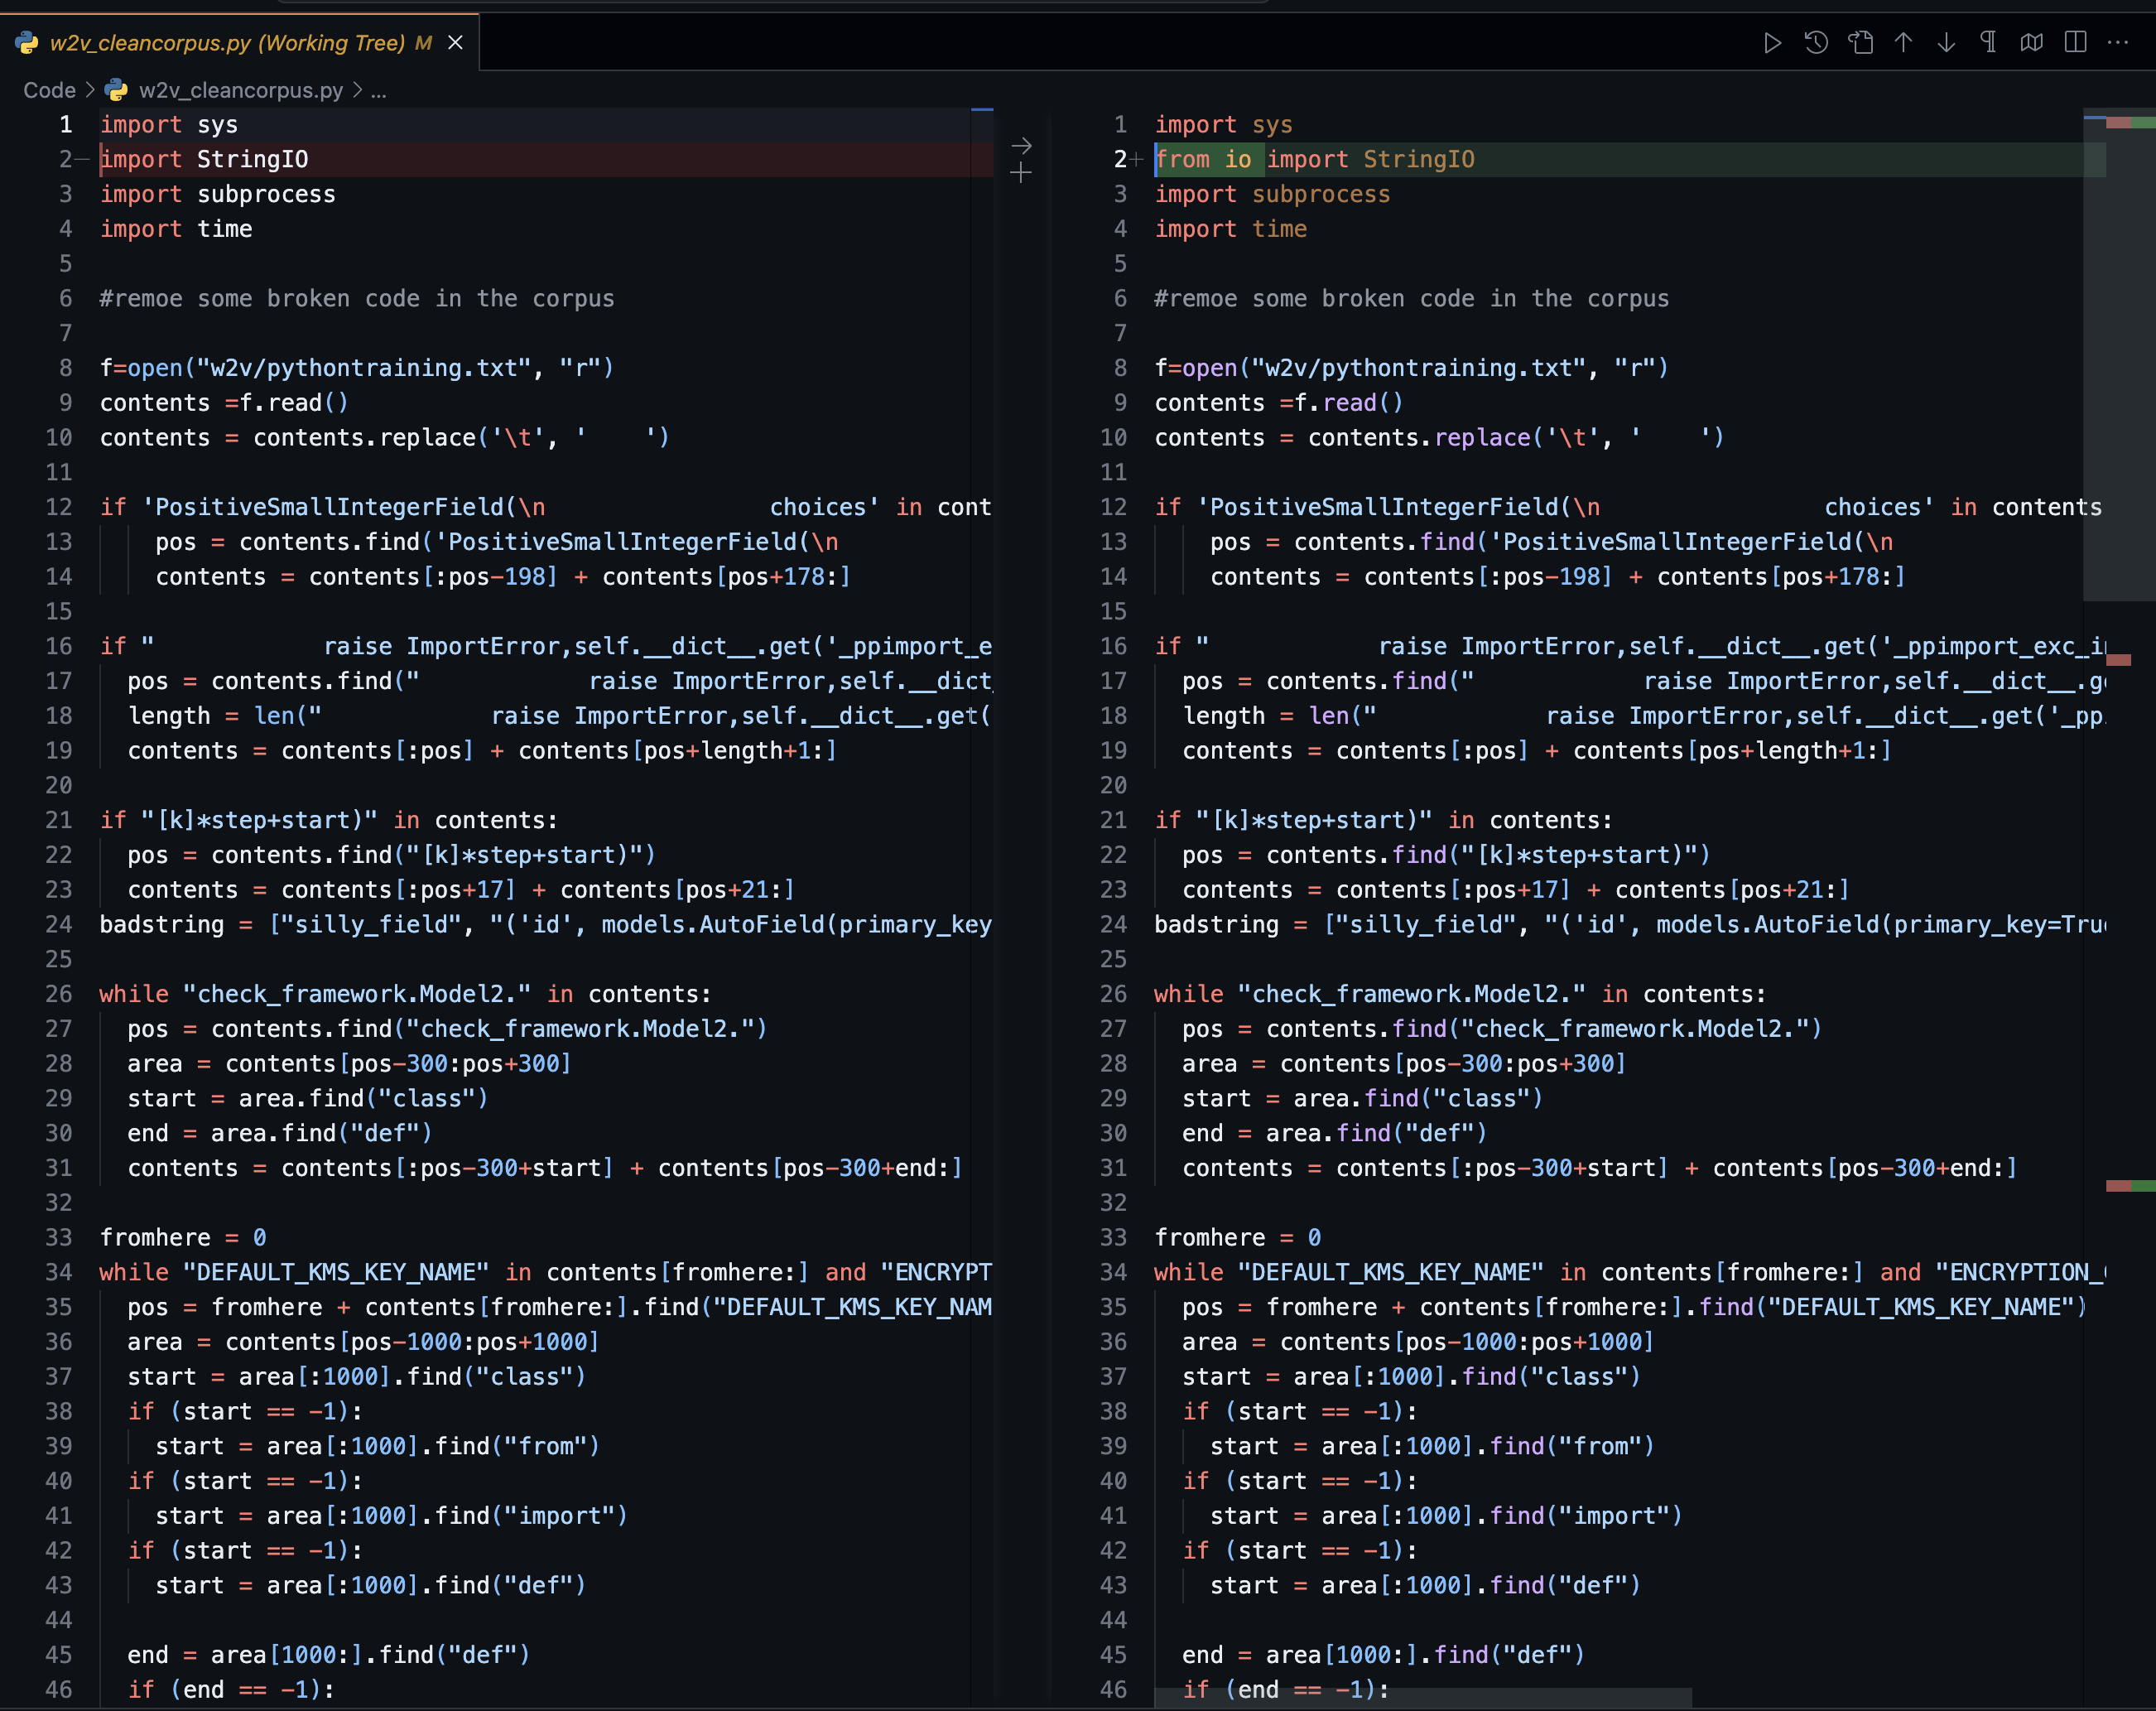
\includegraphics[width=1\linewidth]{pictures/cleancorpus_error.png}
    \caption{Cleancorpus file Issue}
    \label{fig: Figure2}
\end{figure}

After cleaning the mined data, the results are saved in the "pythontraining\_edit.txt". It is shown in Figure \ref{fig: Figure3}
\begin{figure}[!ht]
    \centering
    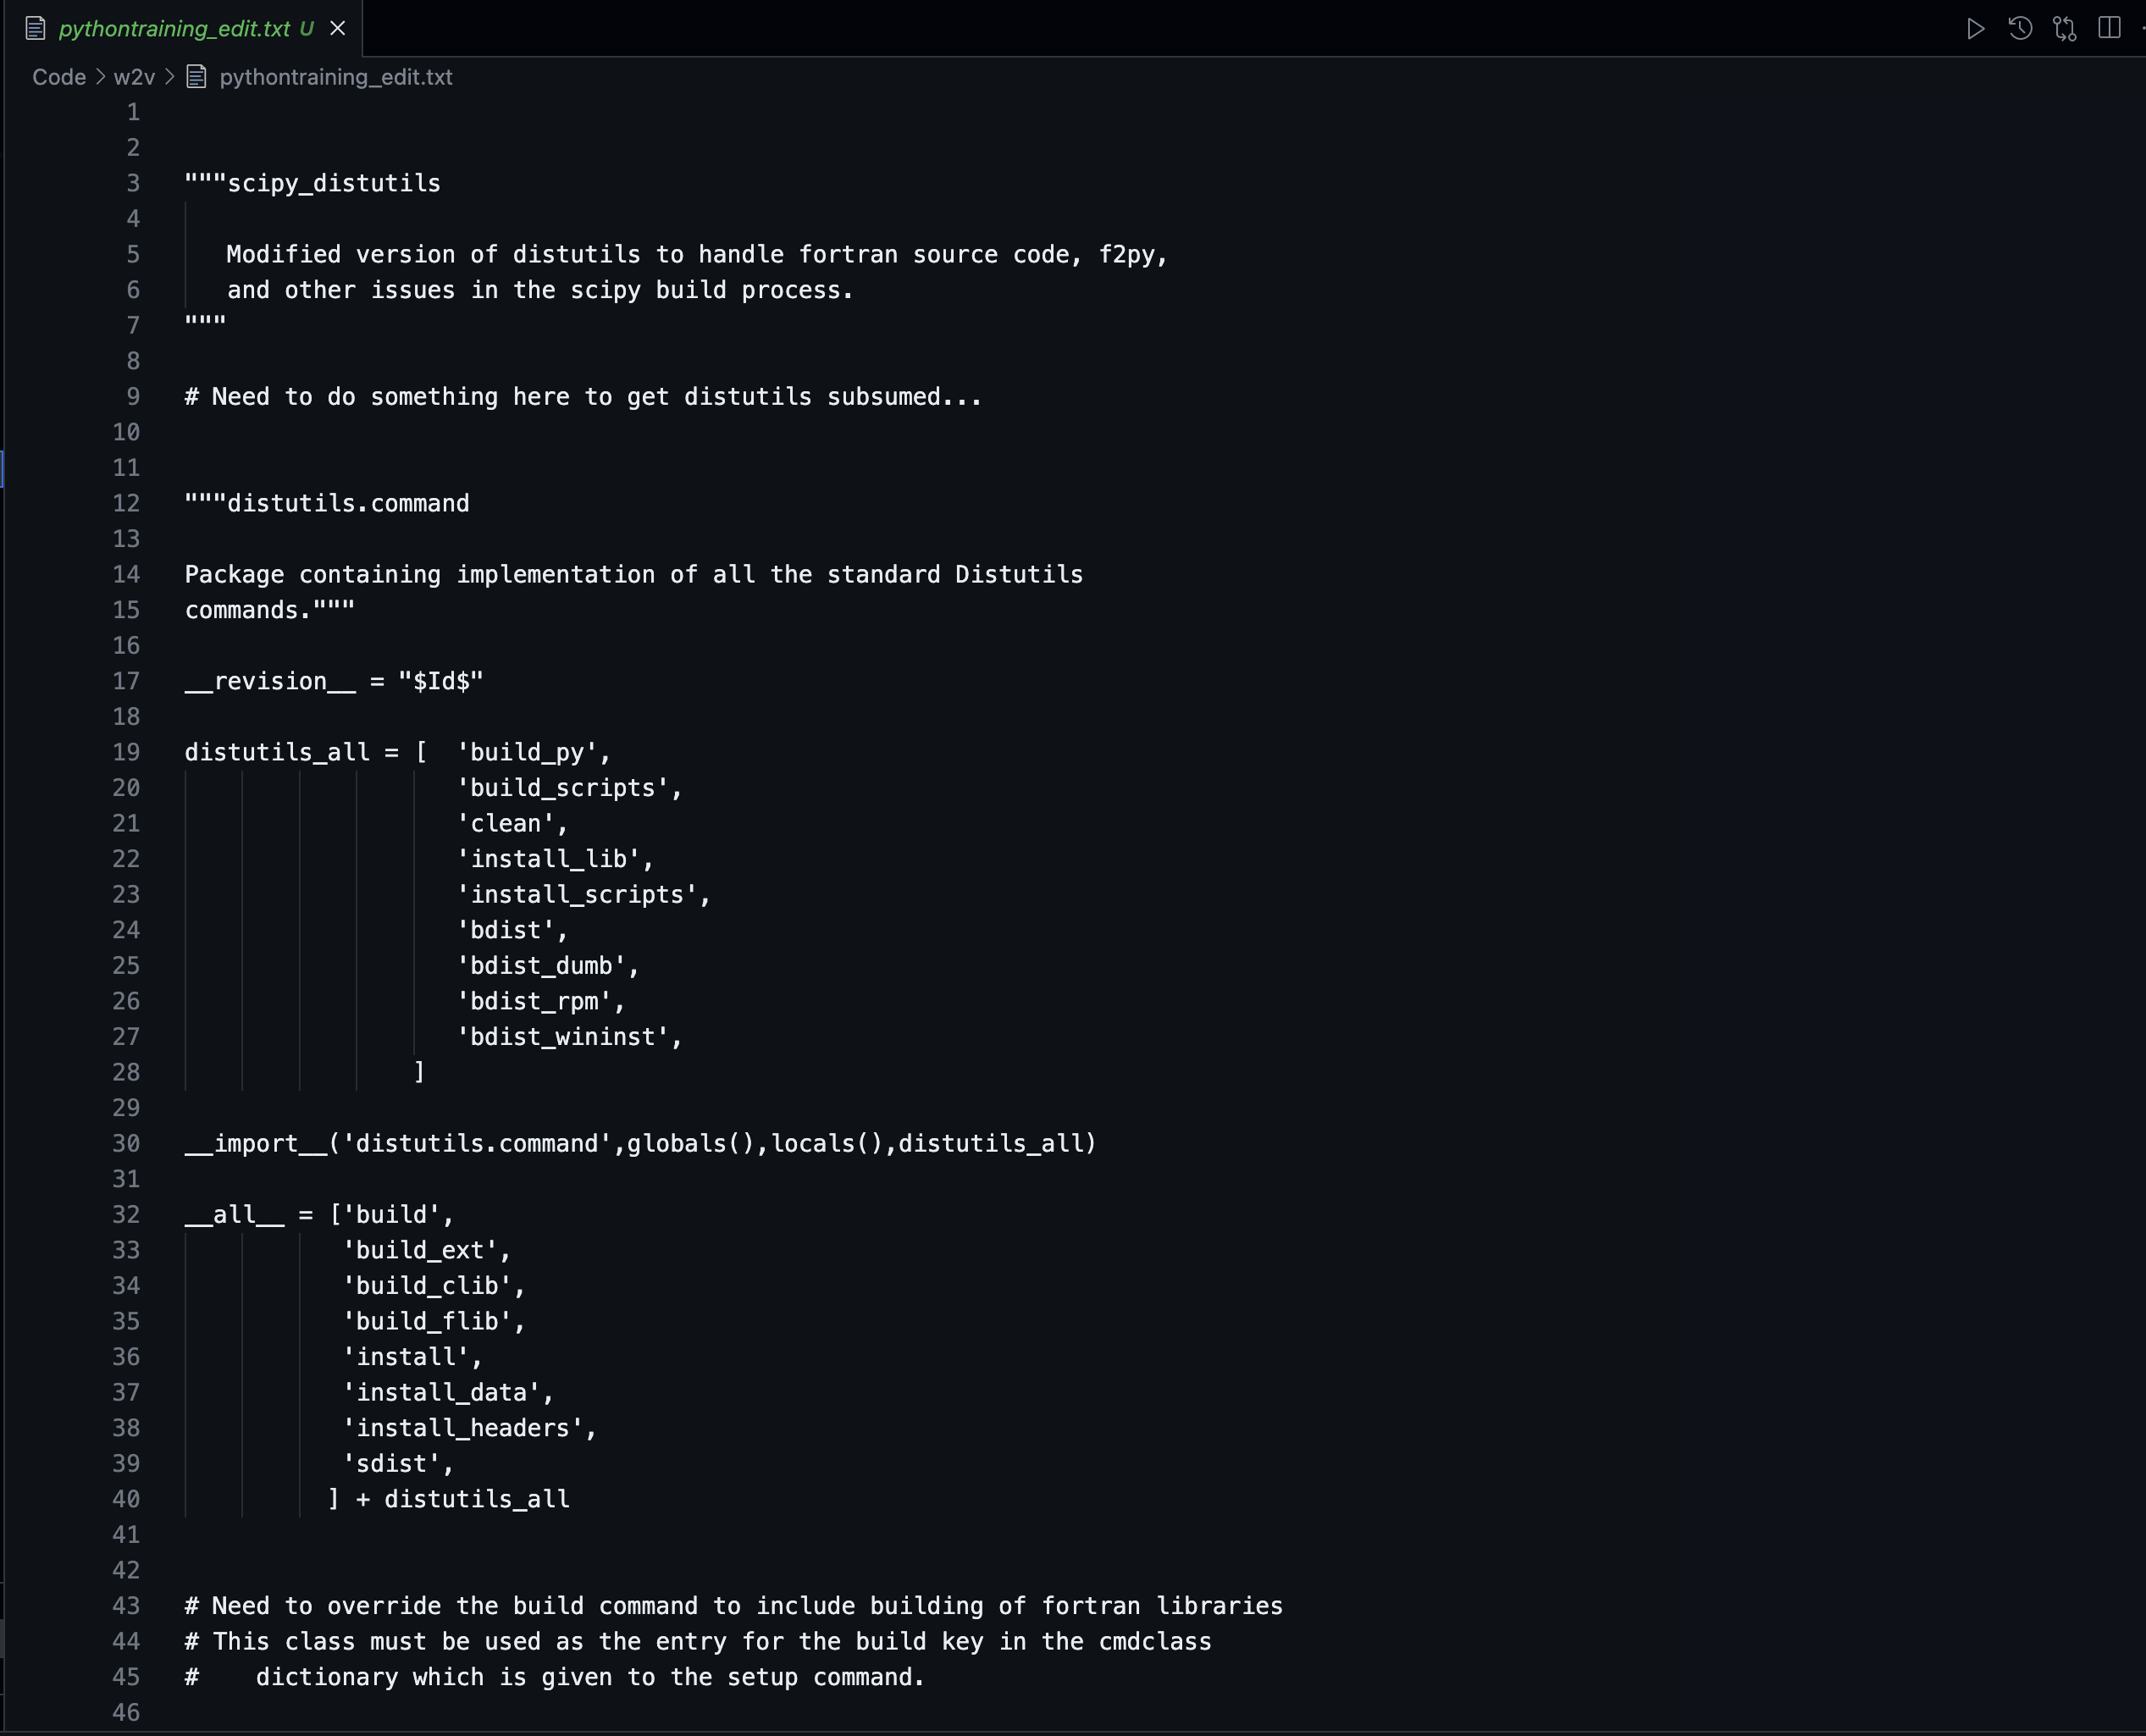
\includegraphics[width=1\linewidth]{pictures/cleaned_data.png}
    \caption{Cleaned Mined Data}
    \label{fig: Figure3}
\end{figure}

\subsection{\textbf{Tokenization}}
Tokenization is one of the essential steps; while using it, we have faced two issues. They are shown in Figure \ref{fig: Figure4}. 
\begin{enumerate}
    \item \textbf{"StringIO" to "io" as a submodule. }\newline When working with text data in Python, especially when dealing with files or streams, the "io" module provides a range of classes and functions to handle input and output operations. "StringIO" is a class in the "io" module that allows you to treat strings as file-like objects. However, if you need to convert the contents of a "StringIO" object to a regular string, you can use the \textit{.getvalue()} method.
    \item \textbf{"\textit{StringIO.StringIO(out)}" method to "\textit{StringIO(out.decode('utf-8'))}"} \newline In Python 3, the StringIO class is located in the io module, and it works with Unicode strings by default. If you have data in bytes format (encoded in UTF-8, for example) and you want to work with it as a string, you need to decode it into a Unicode string. You can achieve this by using the decode() method with the appropriate encoding, in this case, 'utf-8'.
\end{enumerate}

\begin{figure}[!ht]
    \centering
    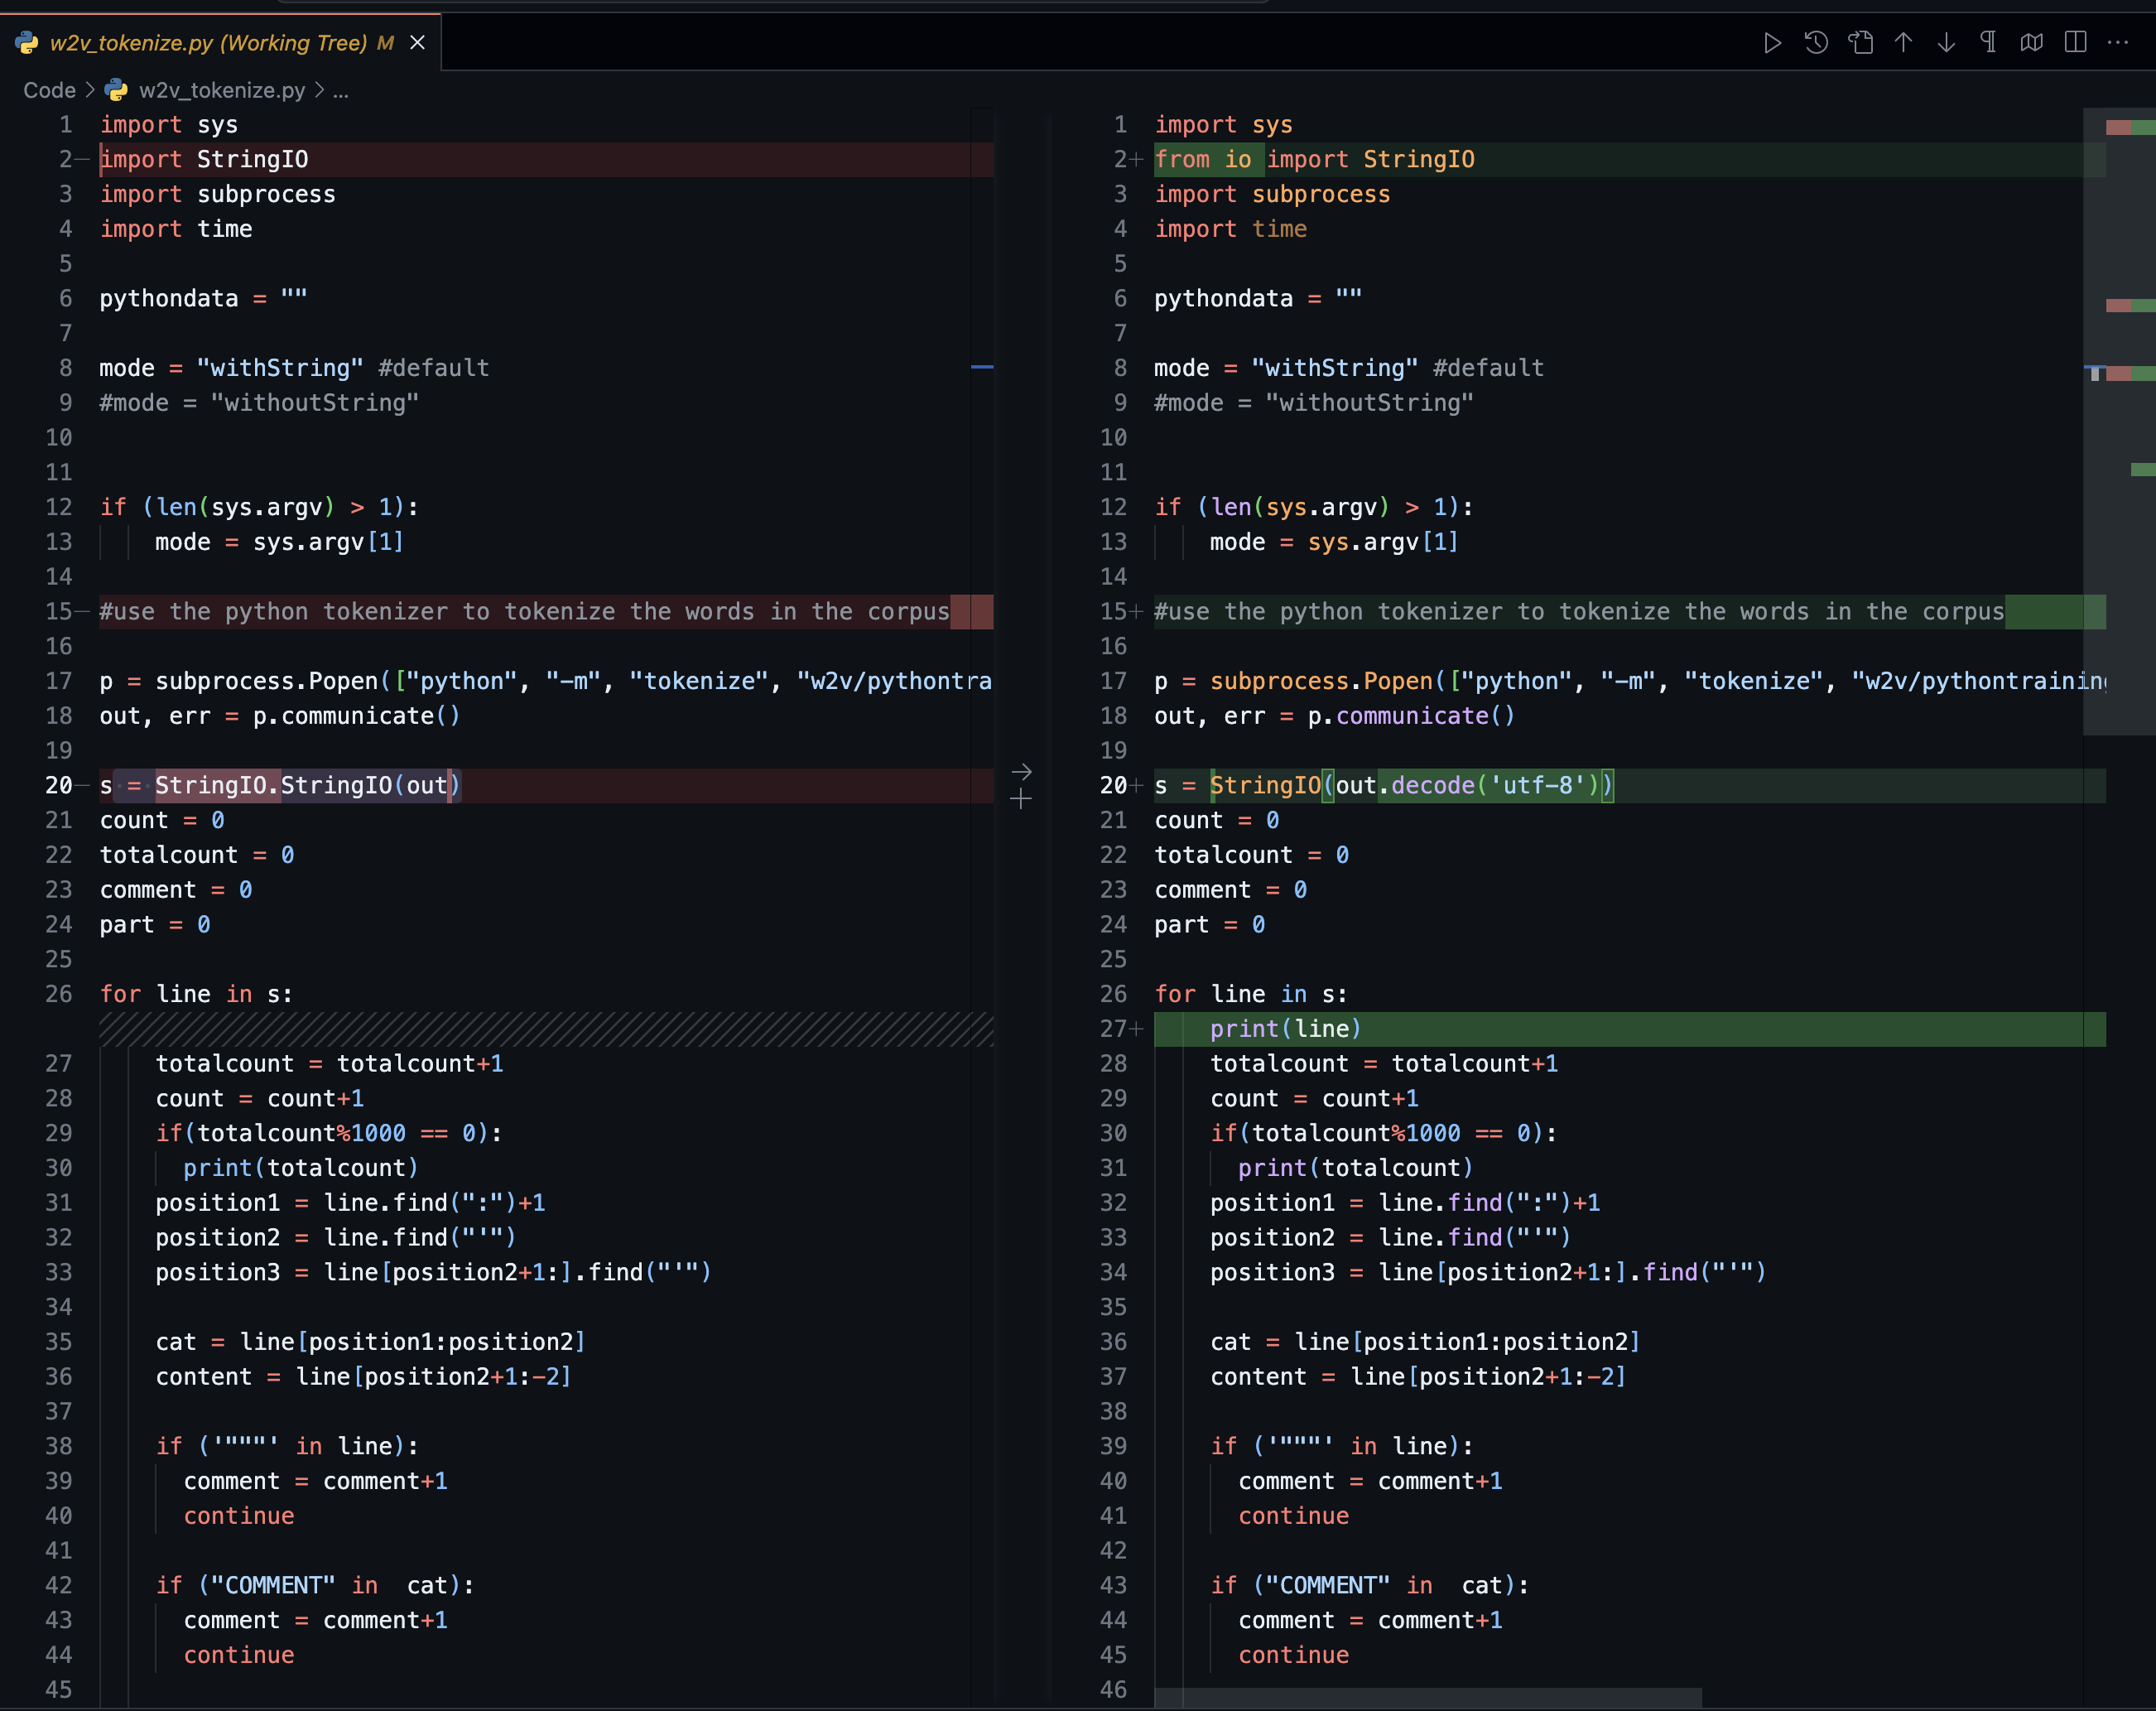
\includegraphics[width=1\linewidth]{pictures/tokenization_isseus.png}
    \caption{Tokenizer issues and solutions}
    \label{fig: Figure4}
\end{figure}

After solving them, we managed to generate the tokenized file. Because of its size, the tokenizer class is divided into 11 files. The saved files are shown in figure \ref{fig: Figure5}.
\begin{figure}[!ht]
    \centering
    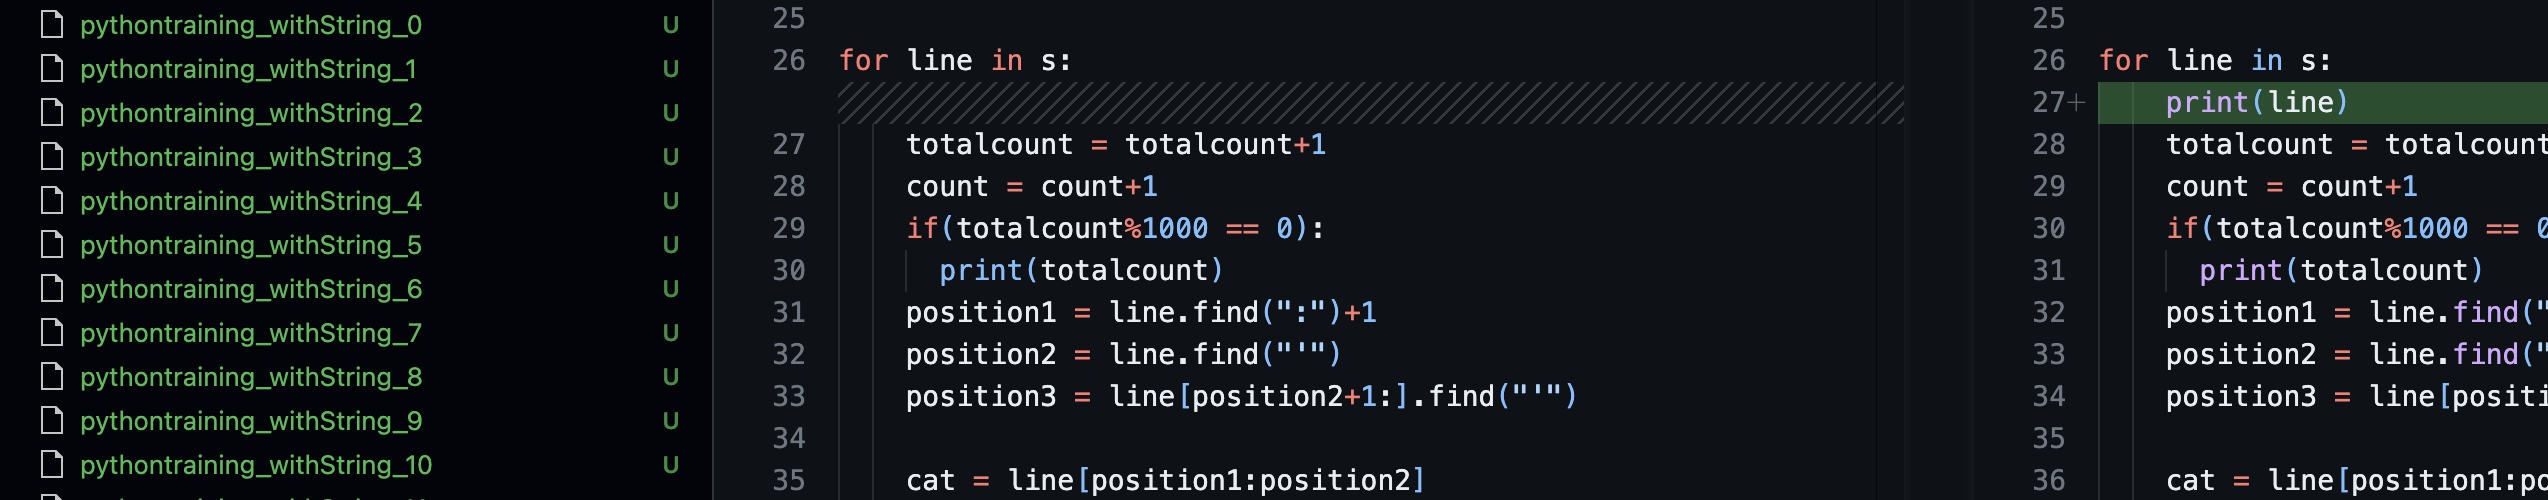
\includegraphics[width=1\linewidth]{pictures/tokenized_data.png}
    \caption{Tokenized data in separate files}
    \label{fig: Figure5}
\end{figure}

\begin{figure}
    \centering
    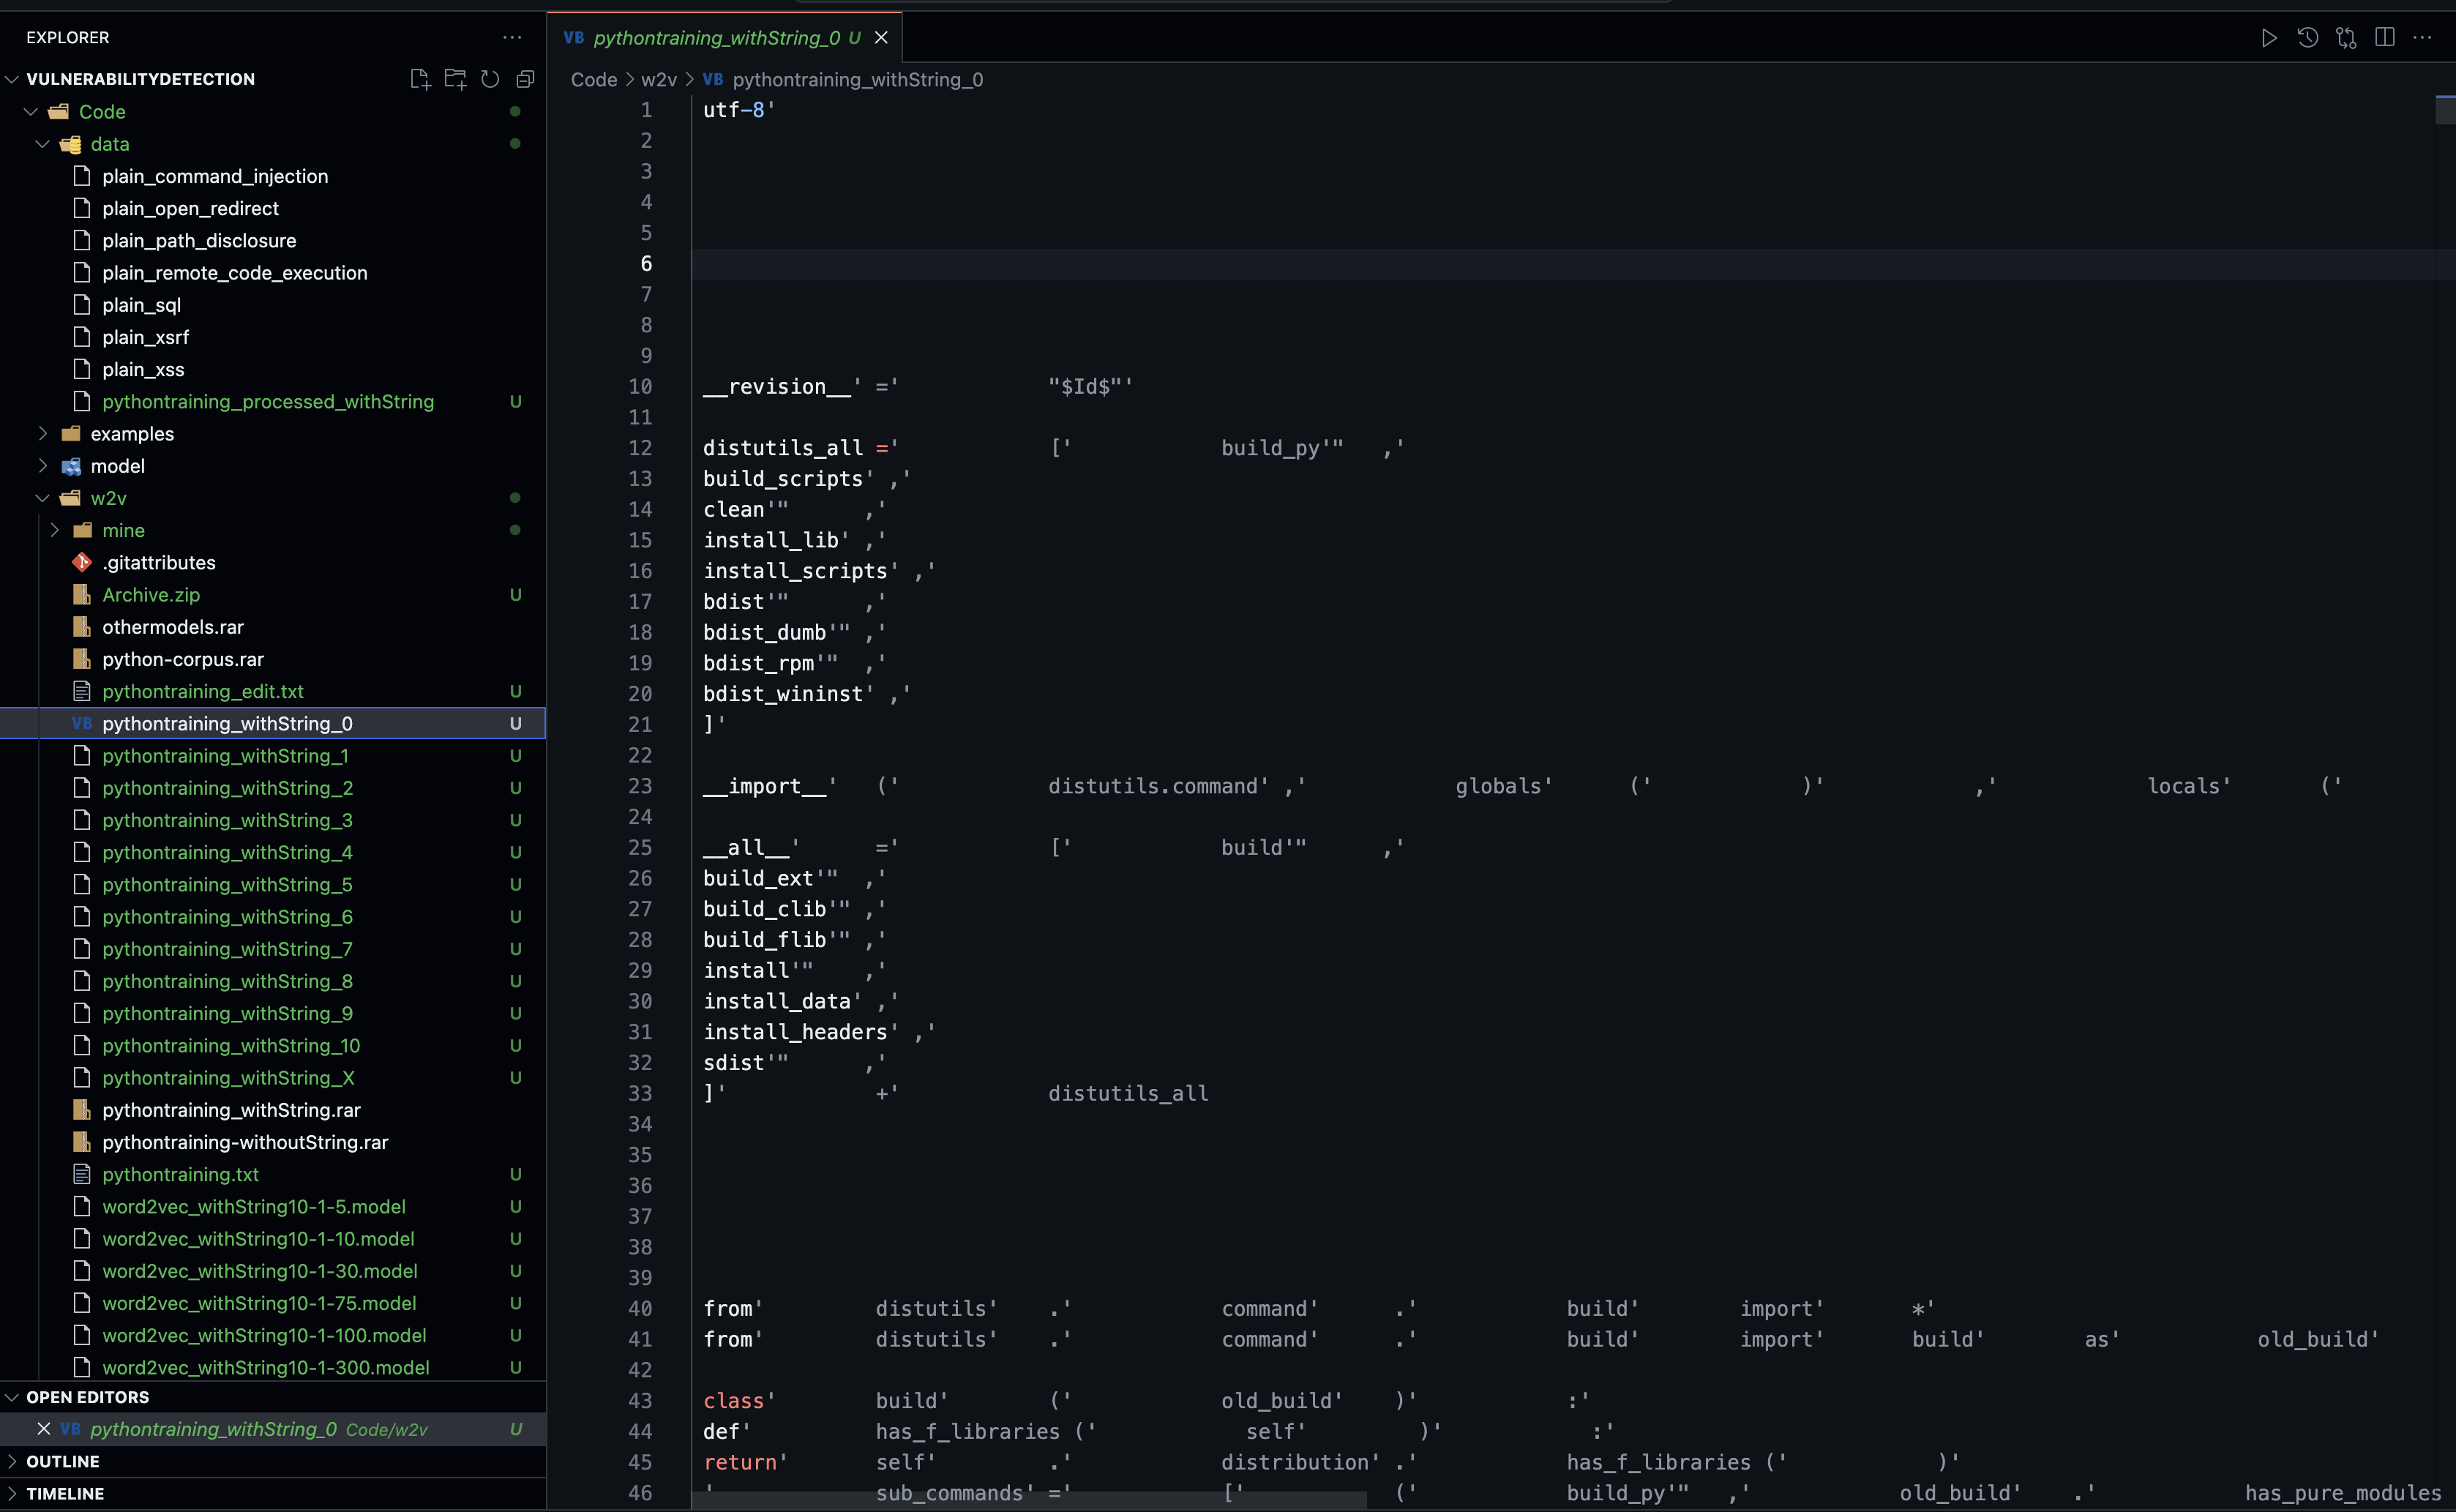
\includegraphics[width=1\linewidth]{pictures/tokenized_sample.png}
    \caption{Tokenized file sample}
    \label{fig: tokenize_sample}
\end{figure}

\subsection{\textbf{Merging Results}}
In this step, you can merge all tokenized data into one large file, which can be beneficial for training your model in the next step. To differentiate this large file from the individual tokenized files, "X" is appended to the end of its name.

While working with this file, we have faced with two issues:
\newline
\begin{enumerate}
 \item The "mode" data variable is missing. This variable saves the mode of tokenization, which has two values (WithString, WithoutString); we have used "WithString" as an exercise file description. We solved this issue by initializing the "mode" variable and assigning the value.
 \item The for loop value range from 0 to 71 was incorrect because we only needed a range of 0 to 10.  We have updated the code and added an exception. Whenever the program does not find the value, it will stop the loop and return the file with "X" at the end of it. Overall changes in this file are shown in Figure \ref{fig: Figure6}
\end{enumerate}

\begin{figure}
    \centering
    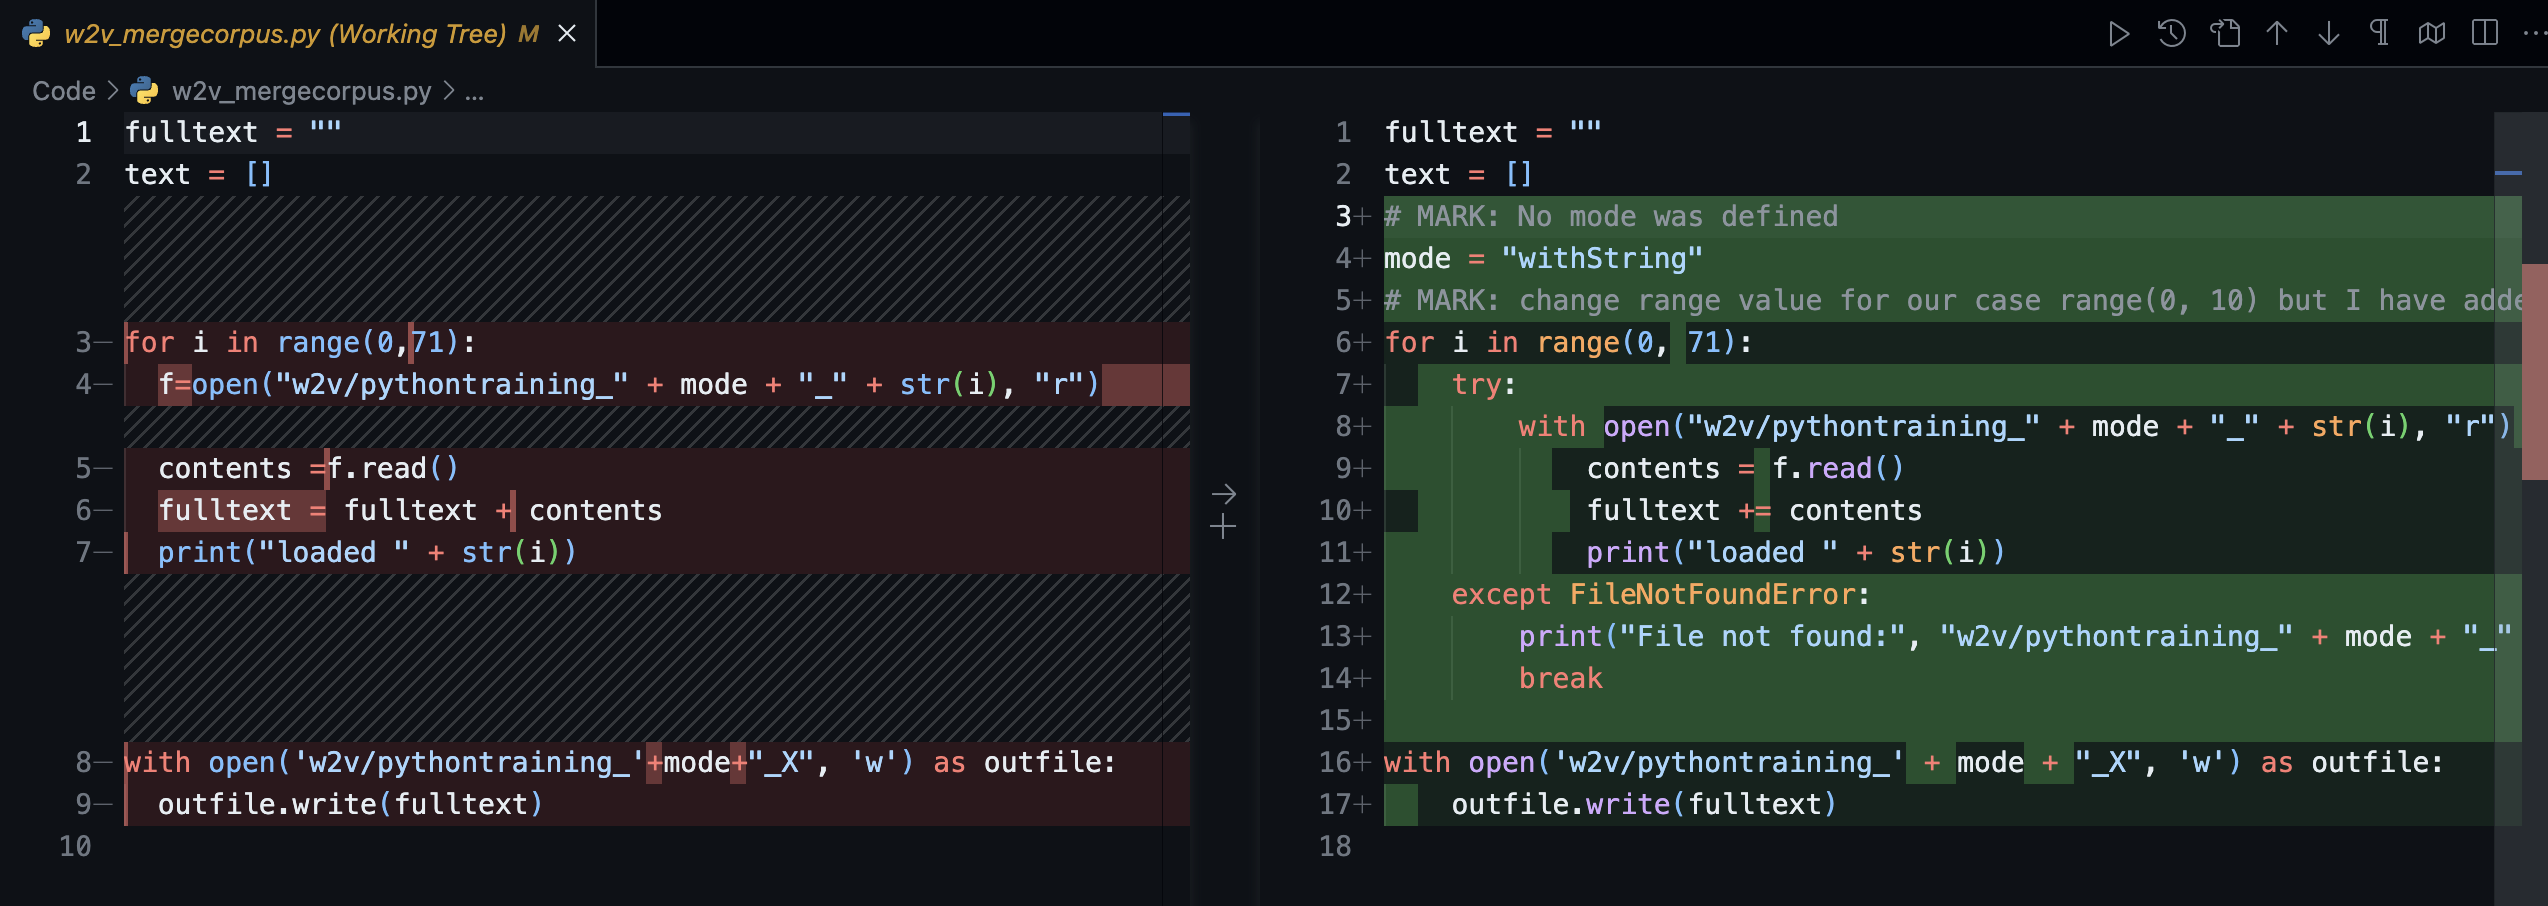
\includegraphics[width=1\linewidth]{pictures/mergin_issues.png}
    \caption{Merging file issues with solutions}
    \label{fig: Figure6}
\end{figure}

After successfully running the file, all 11 tokenized files merged into a large file and received the output. The output has been saved in the "pythontraining\_withString\_X" file, shown in \ref{fig: Figure7}.
\begin{figure}
    \centering
    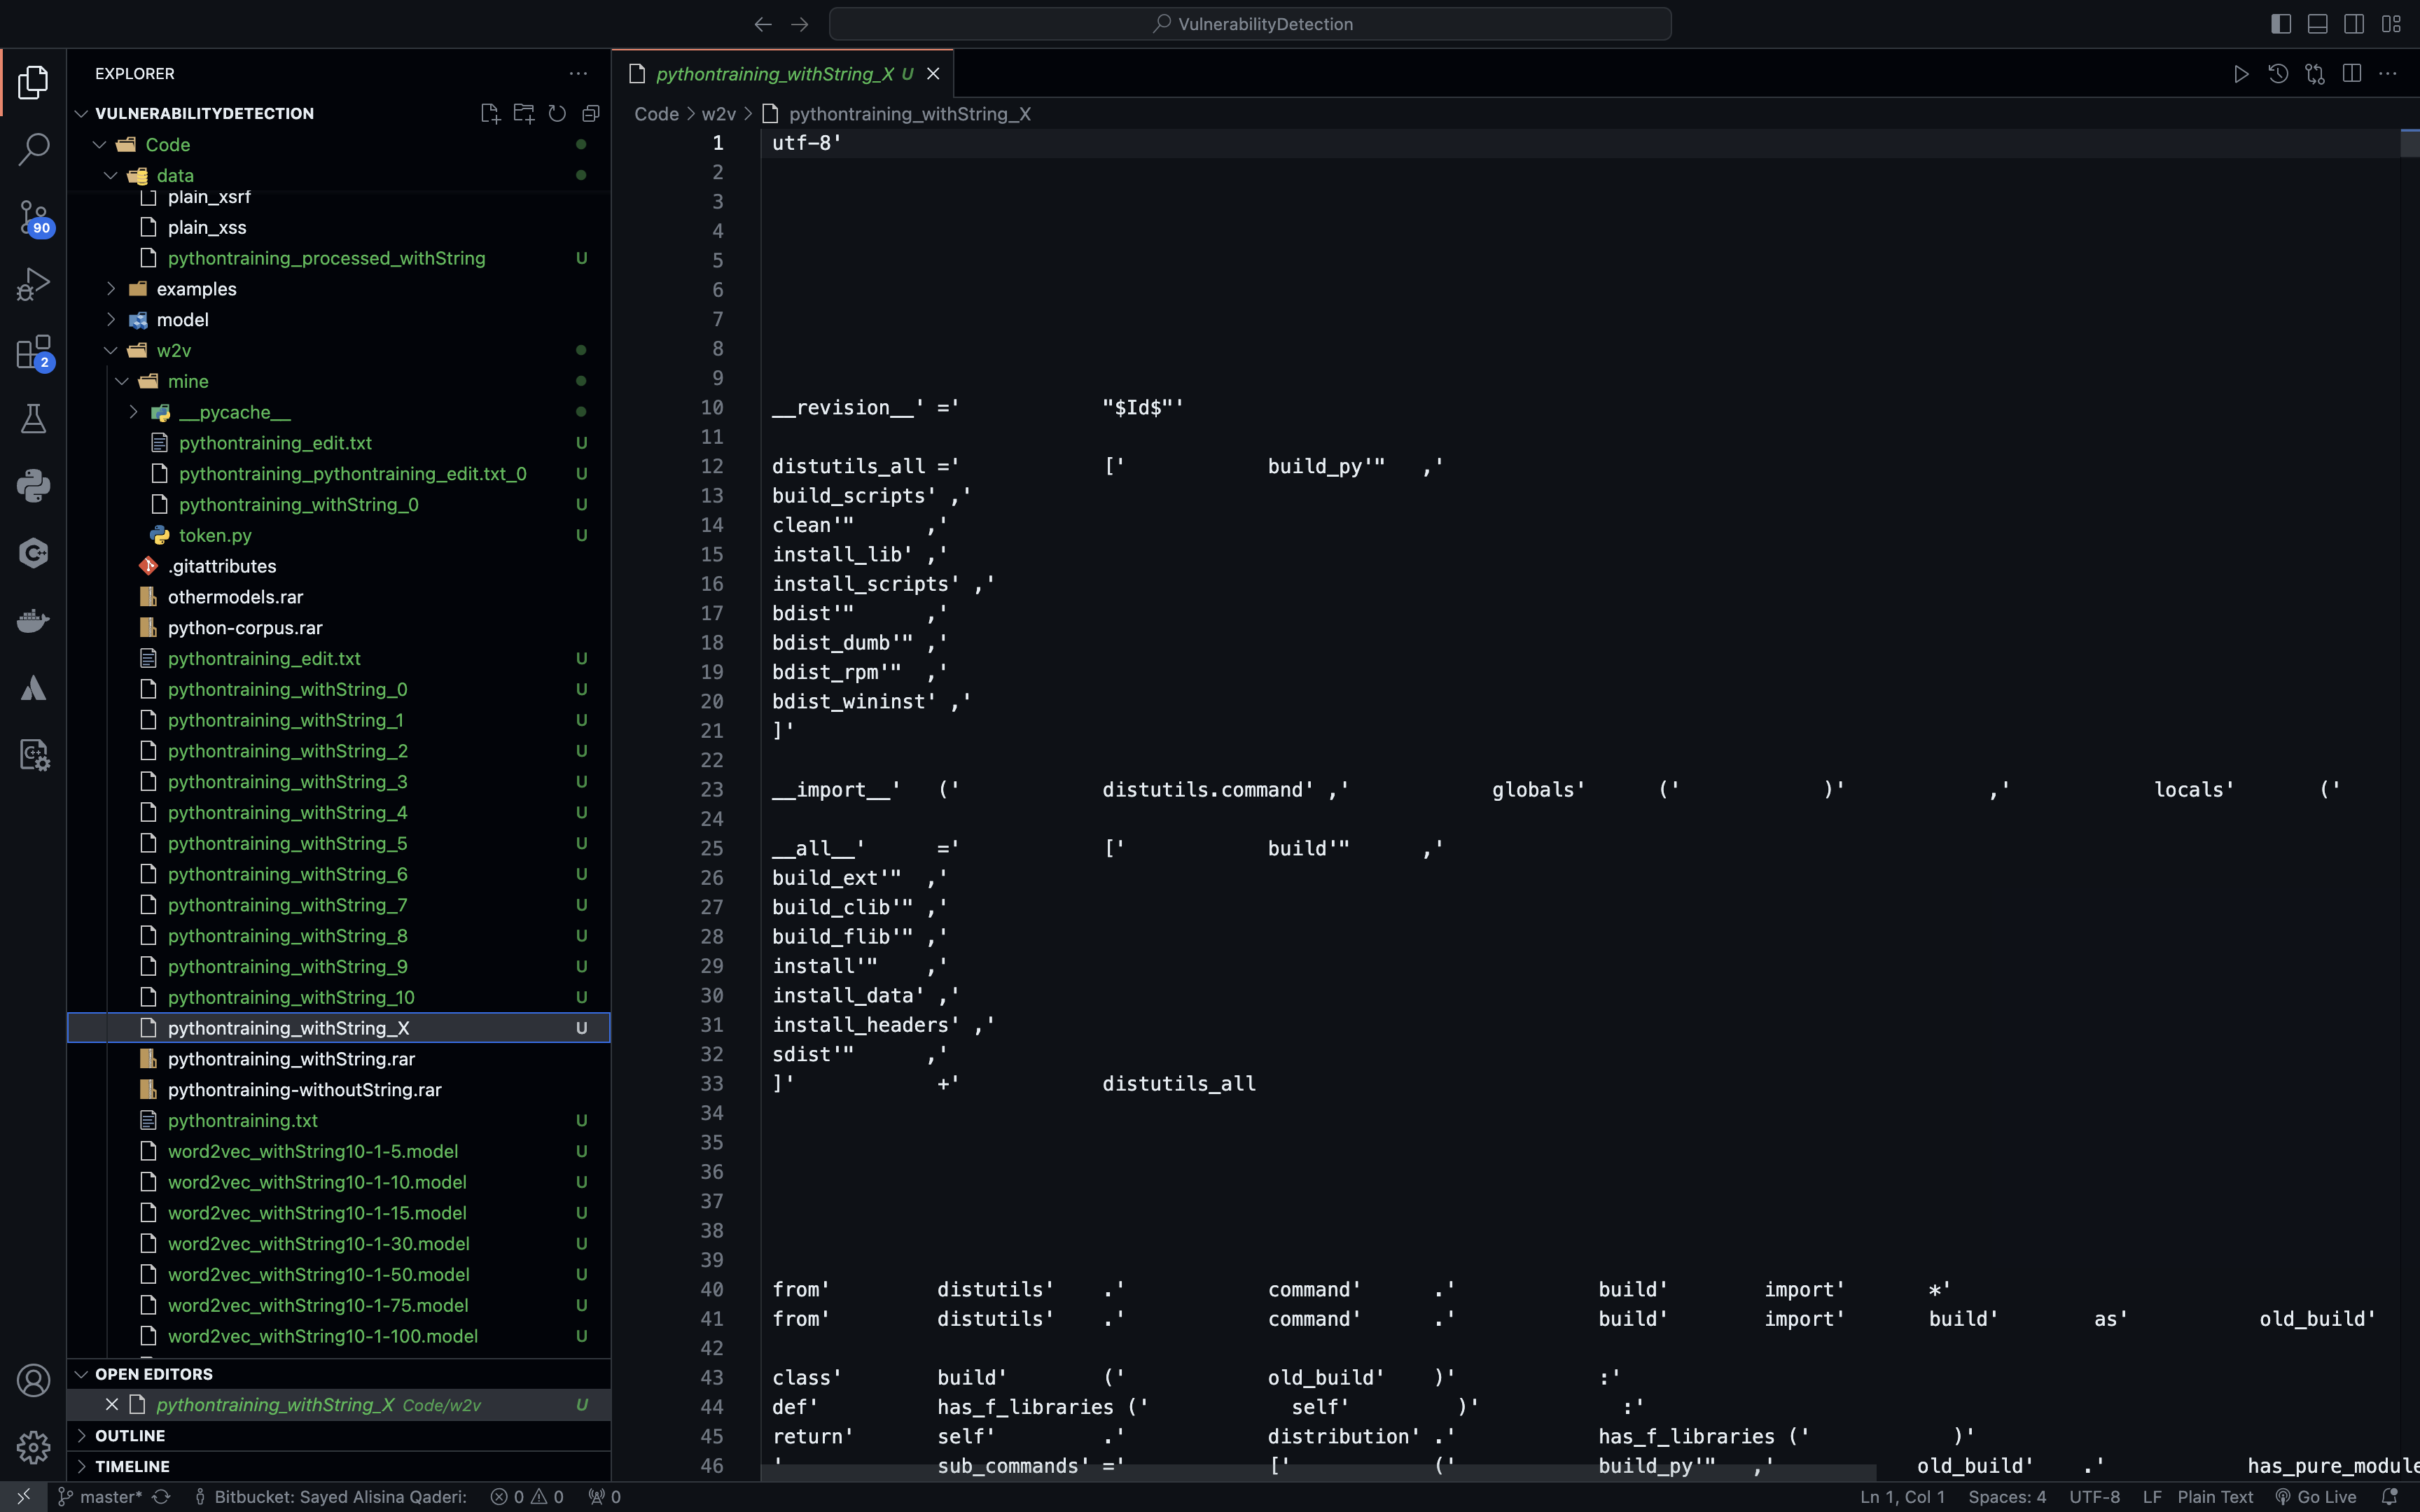
\includegraphics[width=1\linewidth]{pictures/merged_files.png}
    \caption{Merged file}
    \label{fig: Figure7}
\end{figure}

\subsection{\textbf{Training Word2Vec Model}}
In this step, we will generate our model based on tokenized data. While working on this step, we faced some coding issues, which we will explain.
\begin{enumerate}
\item This step required the NLTK library. NLTK has built-in support for dozens of corpora and trained models. To install this library, we should use the following command in the terminal:
    \begin{enumerate}
        \item Mac/Unix: \textit{pip install --user -U nltk}
        \item Windows (32 bit): \textit{pip install nltk} 
        \item As Third Party Software check the following link: \newline \href{https://github.com/nltk/nltk/wiki/Installing-Third-Party-Software}{https://github.com/nltk/nltk/wiki/Installing-Third-Party-Software}
    \end{enumerate}
    After installing the NLTK package, please install the necessary datasets/models for specific functions to work.
    If you’re unsure of which datasets/models you’ll need, you can install the “popular” subset of NLTK data on the command line type \verb |python -m nltk.downloader popular|, or in the Python interpreter \verb|import nltk; nltk.download('popular')| \cite{nltk}
    
    Also, in our case, we have installed only the "punket" model, which was a missing part from NLTK. We solved the problem with "nltk.download('punkt')."
\item Another issue was the deprecation of the Word2Vec library initialization and the ".vocab" variable. It is shown in Figure \ref{fig: Figure8} which changed to ".index\_to\_key"
\item Based on the task description, we should have one model with \textit{paramcount = 10, iterations = 200, and vector size(s) = 300} parameters. 
\newline The iterations=200 was missing, so we manually added it to the array. It is shown in Figure \ref{fig: Figure9}.
\end{enumerate}
\begin{figure}
    \centering
    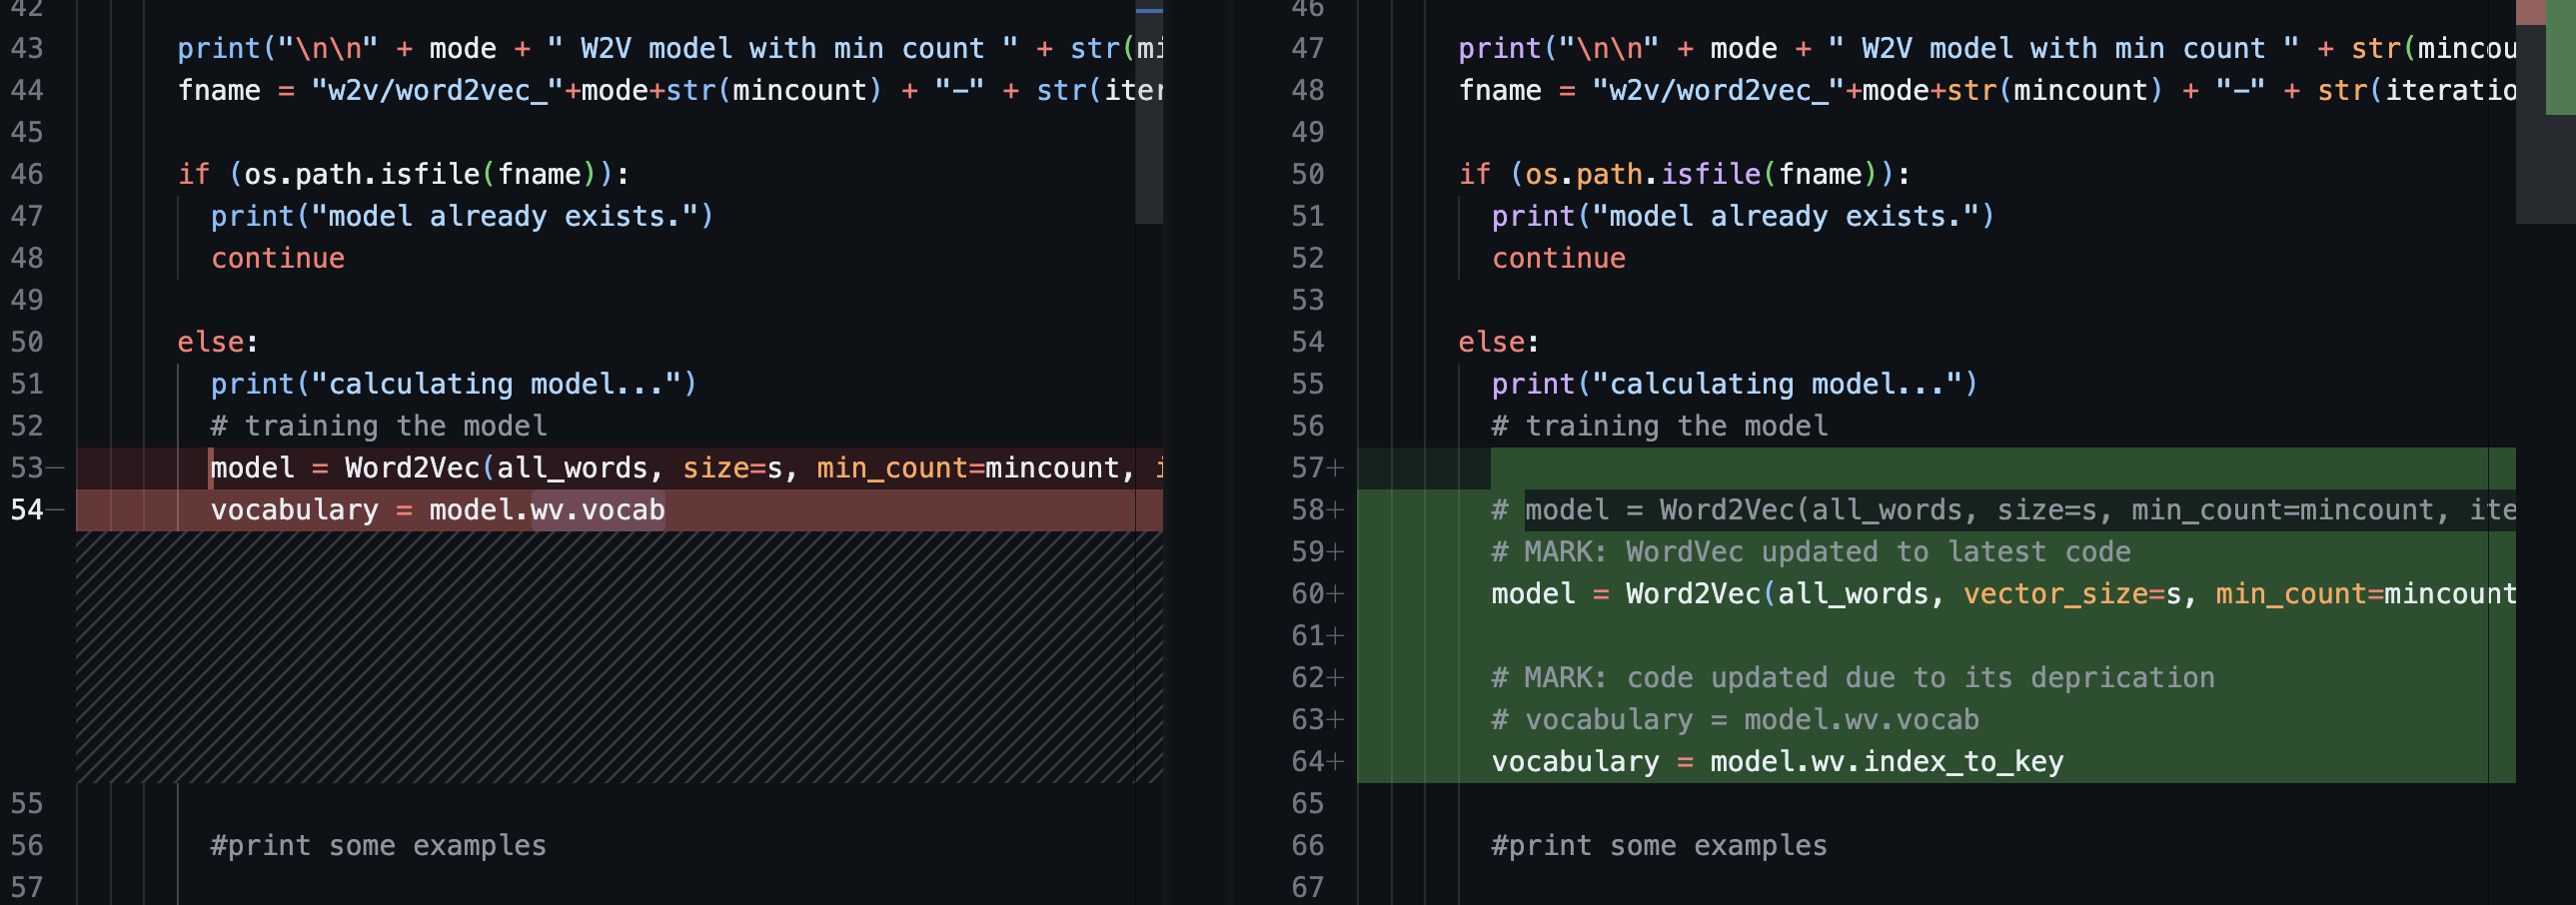
\includegraphics[width=1\linewidth]{pictures/word2vec_deprication.png}
    \caption{Word2Vec Deprecated Code \& Update Code}
    \label{fig: Figure8}
\end{figure}

\begin{figure}
    \centering
    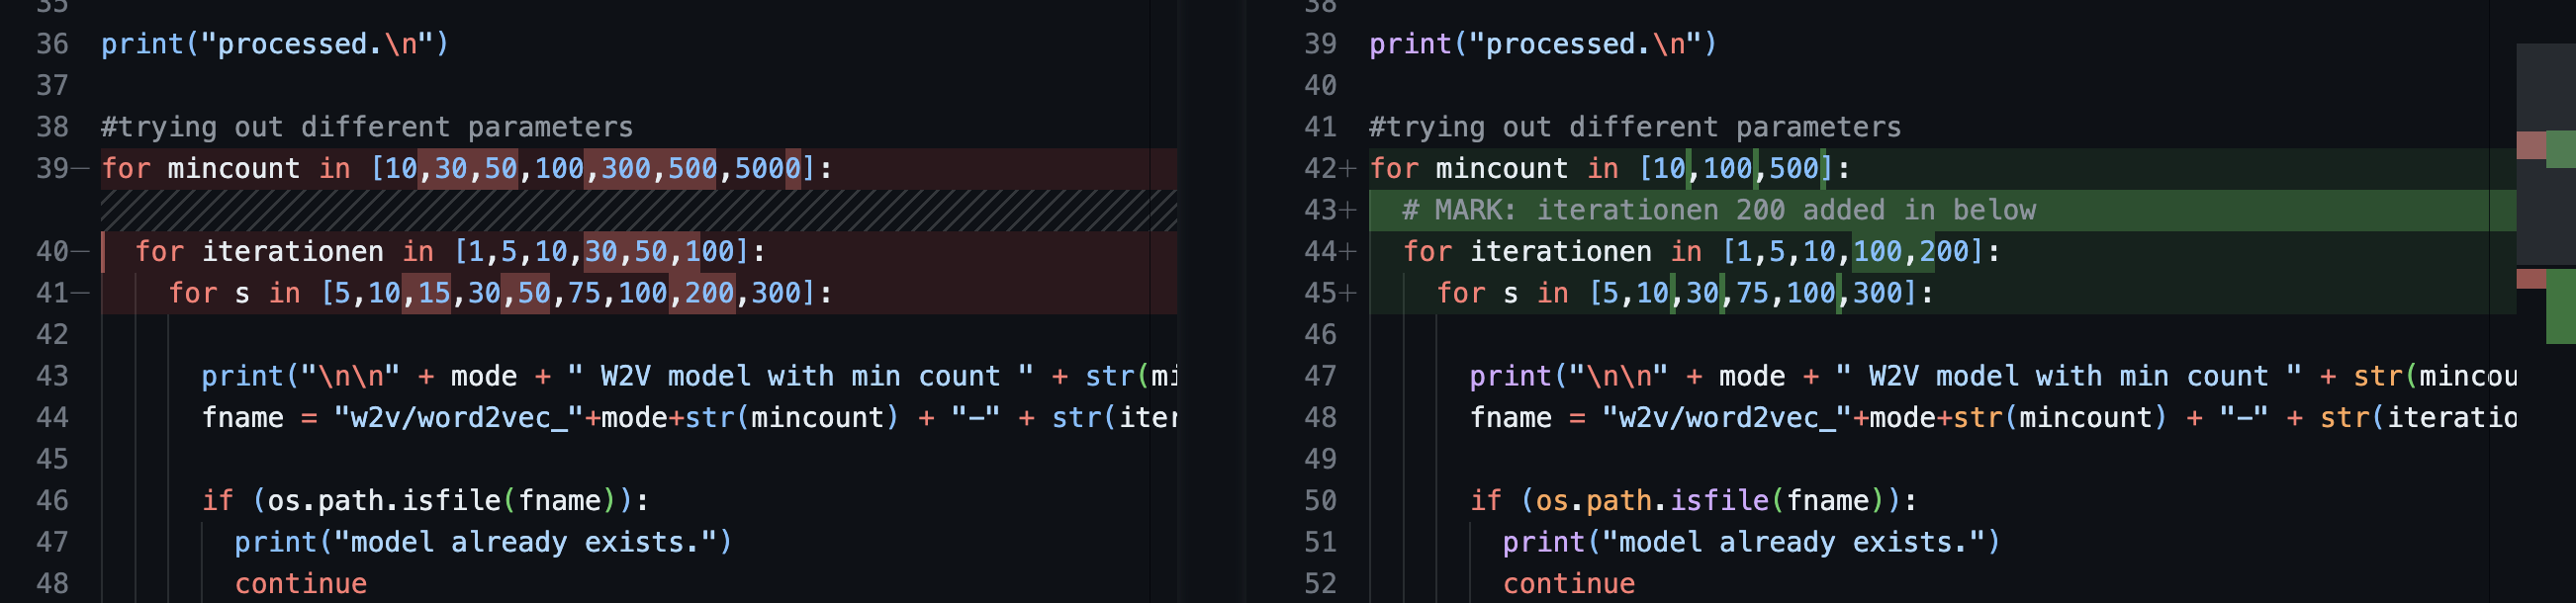
\includegraphics[width=1\linewidth]{pictures/missing_value.png}
    \caption{Missing Iteration Value}
    \label{fig: Figure9}
\end{figure}

After addressing the mentioned issues and implementing the necessary changes, our model training process proceeded successfully with the following parameters (refer to Figure 9):
\begin{itemize}
    \item mincount: [10, 100, 500]
    \item iterations: [1, 5, 10, 100, 200]
    \item vector size (s): [5, 10, 30, 75, 100, 300]
\end{itemize}
These parameters were chosen to optimize our model's performance while considering factors like word frequency thresholds (mincount), training iterations (iterations), and vector size (s).

Additionally, we implemented optimizations to enhance efficiency in both time and space utilization.

As a result of our training, we generated a total of 90 .model files, each representing a trained model. You can observe the model training process in Figure \ref{fig: Figure10}.
\begin{figure}
    \centering
    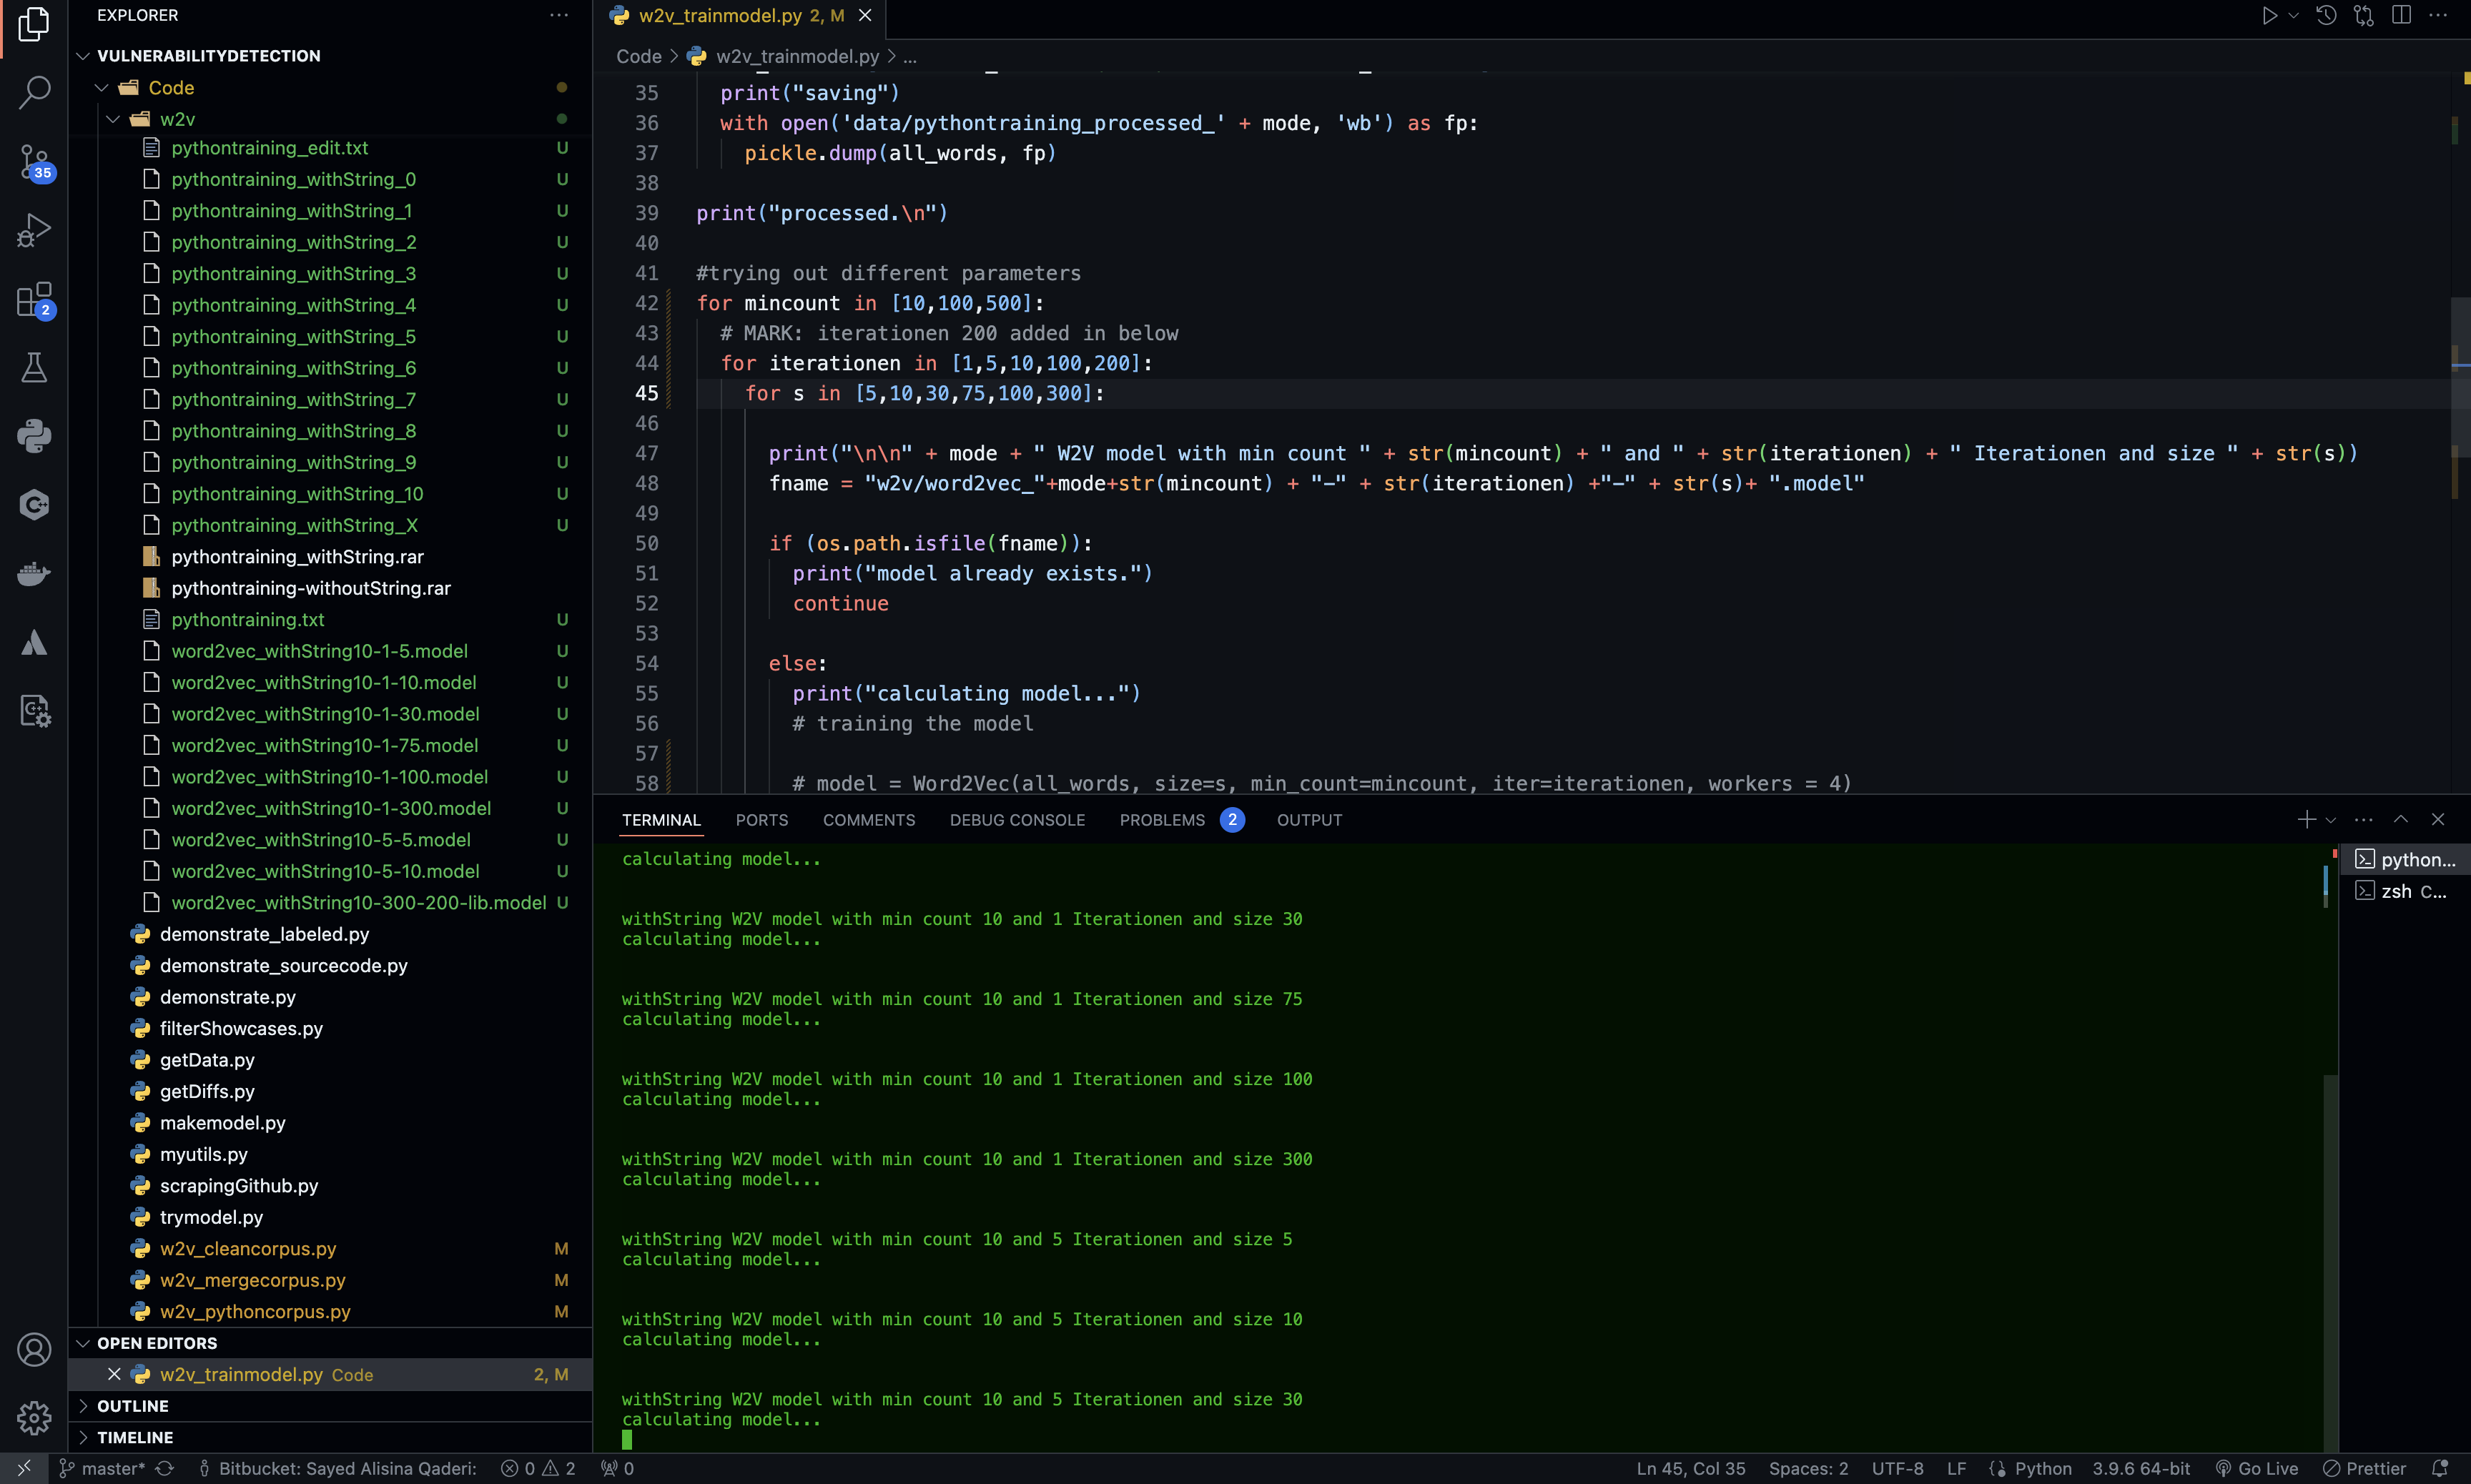
\includegraphics[width=1\linewidth]{pictures/model_training.png}
    \caption{Model Training}
    \label{fig: Figure10}
\end{figure}
\newline
The models will be shared along with this report as archived.


% Bibliography
\clearpage
\bibliographystyle{plainurl}
\bibliography{ref}
\thispagestyle{empty} % Remove the page number from the reference page

\end{document}
